\chapter{The NOvA experiment}\label{sec:NOvA}
%%% OVERVIEW OF THE NOvA EXPERIMENT %%%

The \gls{NOvA} \cite{NOvAWebsite} is a long-baseline neutrino oscillation experiment based at the \gls{Fermilab}
%Fermi National Accelerator Laboratory (Fermilab) 
\cite{FNALWebsite}. \gls{NOvA} receives an off-axis $\nu_\mu$ and $\overline{\nu}_\mu$ beam from \gls{Fermilab}'s \gls{NuMI} neutrino source, described in Sec.~\ref{fig:NOvANuMI}, and measures $\nu_e$/$\overline{\nu}_e$ appearance and $\nu_\mu$/$\overline{\nu}_\mu$ disappearance between its two highly active and finely segmented detectors, described in Sec.~\ref{fig:NOvADetectors} \cite{PhysicsOfNOvA.pdf}. 

The capability to measure both $\nu_e$ and $\overline{\nu}_e$ appearance, coupled with a significant matter effect induced by the long baseline, allows \gls{NOvA} to address some of the most important questions in neutrino physics to date, such as the neutrino mass ordering, the octant of $\theta_{23}$, and the possible \gls{CP} violation in the neutrino sector \cite{PhysicsOfNOvA.pdf,NOvAStatusAndOutlook.pdf,FirstNOvAResult.pdf,2019NOvAFHCRHCResults.pdf,NOvAResults2021.pdf}. \gls{NOvA} data also enables measurements of the values of $\theta_{13}$, $\theta_{23}$ and $\left|\Delta m^2_{atm}\right|$ \cite{PhysicsOfNOvA.pdf}, measurements of neutrino differential cross sections in the near detector \cite{NOvANCPi0XSecMeasurement2019.pdf, NOvANumuCCXSexMeasurement2023.pdf, NOvANueCCXSecMeasurement2023.pdf, NOvANuMuCCPi0XSecMeasurement2023.pdf}, constraints on the possible sterile neutrino models \cite{NOvASterilesFHCResults2017.pdf, NOvASterilesFHCRHCResults2021.pdf}, monitoring for supernova neutrino activity \cite{NOvASupernovaMeasurements2020.pdf, NOvASupernovaCoincidenceMeasurements2021.pdf}, searches for magnetic monopoles \cite{NOvASlowMagMonopoles2021.pdf}, and constraints on the neutrino electromagnetic properties (this thesis). Using two functionally identical detectors mitigates the systematic uncertainties of neutrino oscillation measurements, described in Sec.~\ref{sec:NOvASystematics}.

%\note{Should I mention here when did NOvA start taking data and how long is it planning to run for? Maybe future analysis? Size of the collaboration? - YES!}

\gls{NOvA} started taking data in February 2014 and is expected to run through 2026 \cite{NOvAHalfTimeOverview2022.pdf}.
\todo{Add DUNE into this and find the LOI reference}

%From NOvAHalfTimeOverview2022.pdf: NOvA started physics data-taking with the first 5 kt of the far detector in February 2014, and saw the completion of the near and far detectors completed later that year. Annual beam exposure, measured in protons-on-target (POT) to NuMI ramped up as the design beam power for NOvA of 700 kW was achieved in 2017. Further improvements to the NuMI target system now allow even higher power, with a record 1 hour average power of 843 kW. As of May 2021, the far detector has recorded data for nearly 17 × 1020 POT delivered to NuMI in neutrino mode, when weighting data collected during construction for the fraction of the detector active at the time, and 12.7 × 1020 POT delivered in antineutrino mode. NOvA expects to continue data-taking until 2026 and hopes to double the current exposure in both neutrinos and antineutrinos.
%NOvA is expected to take data through 2026 [67], when the Fermilab accelerator complex is shutdown for construction of the Long-Baseline Neutrino Facility (LBNF) for DUNE. During the remaining running time, the beam power delivered to NuMI should increase. Following installation of additional beam dampers and collimators scheduled in 2023-4 as part of the PIP-II project [68], the Fermilab accelerator complex should be capable of delivering more than 900 kW to NuMI. The ultimate exposure delivered to NuMI will depend on the timeline of the remaining power improvements, other demands on beam from the Main Injector, and the total run length. The current projection is between 60 and 70 × 1020 protons on target.
%With the NOvA test beam effort underway and ongoing improvements to neutrino interaction measurements and modeling, the sensitivity of NOvA to three-flavor oscillation parameters will remain statistics-limited through the end of the experiment [77]. The expected total beam exposure will bring additional compelling milestones into reach. For the Mass Hierarchy, NOvA will achieve 95\% a priori sensitivity for 40-60\% of possible δCP values and 4-5$\sigma$ a priori sensitivity for the most favorable combinations of the true values of the oscillation parameters. For CP-violation, a median, a priori sensitivity of 2-sigma is projected for 20-30\% of the $\delta$CP range. The physics reach of NOvA will be complimented by a joint analysis effort underway between NOvA and T2K [78].
%NOvA has already informed the design of the next generation of neutrino experiments from the insights gained from the performance of its beamline and detectors, and from its experience in operations and development of analysis techniques. NOvA has also informed the neutrino interaction and oscillation landscape with results from across its full portfolio of physics topics, and will continue to do so until the onset of the DUNE and T2HK era.

\section{The Neutrino Beam}\label{sec:NuMI}

The neutrino beam for \gls{NOvA} comes from the \gls{Fermilab}-based \gls{NuMI} neutrino source \cite{NuMI.pdf}. The schematic description of \gls{NuMI} is shown in Fig.~\ref{fig:NOvANuMI}, starting on the left hand side with $\unit[120]{GeV}$ protons from the \gls{MI}, part of the \gls{Fermilab} accelerator complex. The proton beam is divided into $\unit[10]{\mu s}$ long pulses, with $\sim5\times 10^{13}$ \gls{POT} per spill every $\sim\unit[1.3]{s}$ long cycle time, resulting in a proton beam power of $\sim\unit[800]{kW}$, with upgrades currently underway to surpass $\unit[1]{MW}$ \cite{NuMIUpgradeToMWProceedings2022.pdf}.

\begin{figure}[!hbtp]
\centering
%is pdf-a
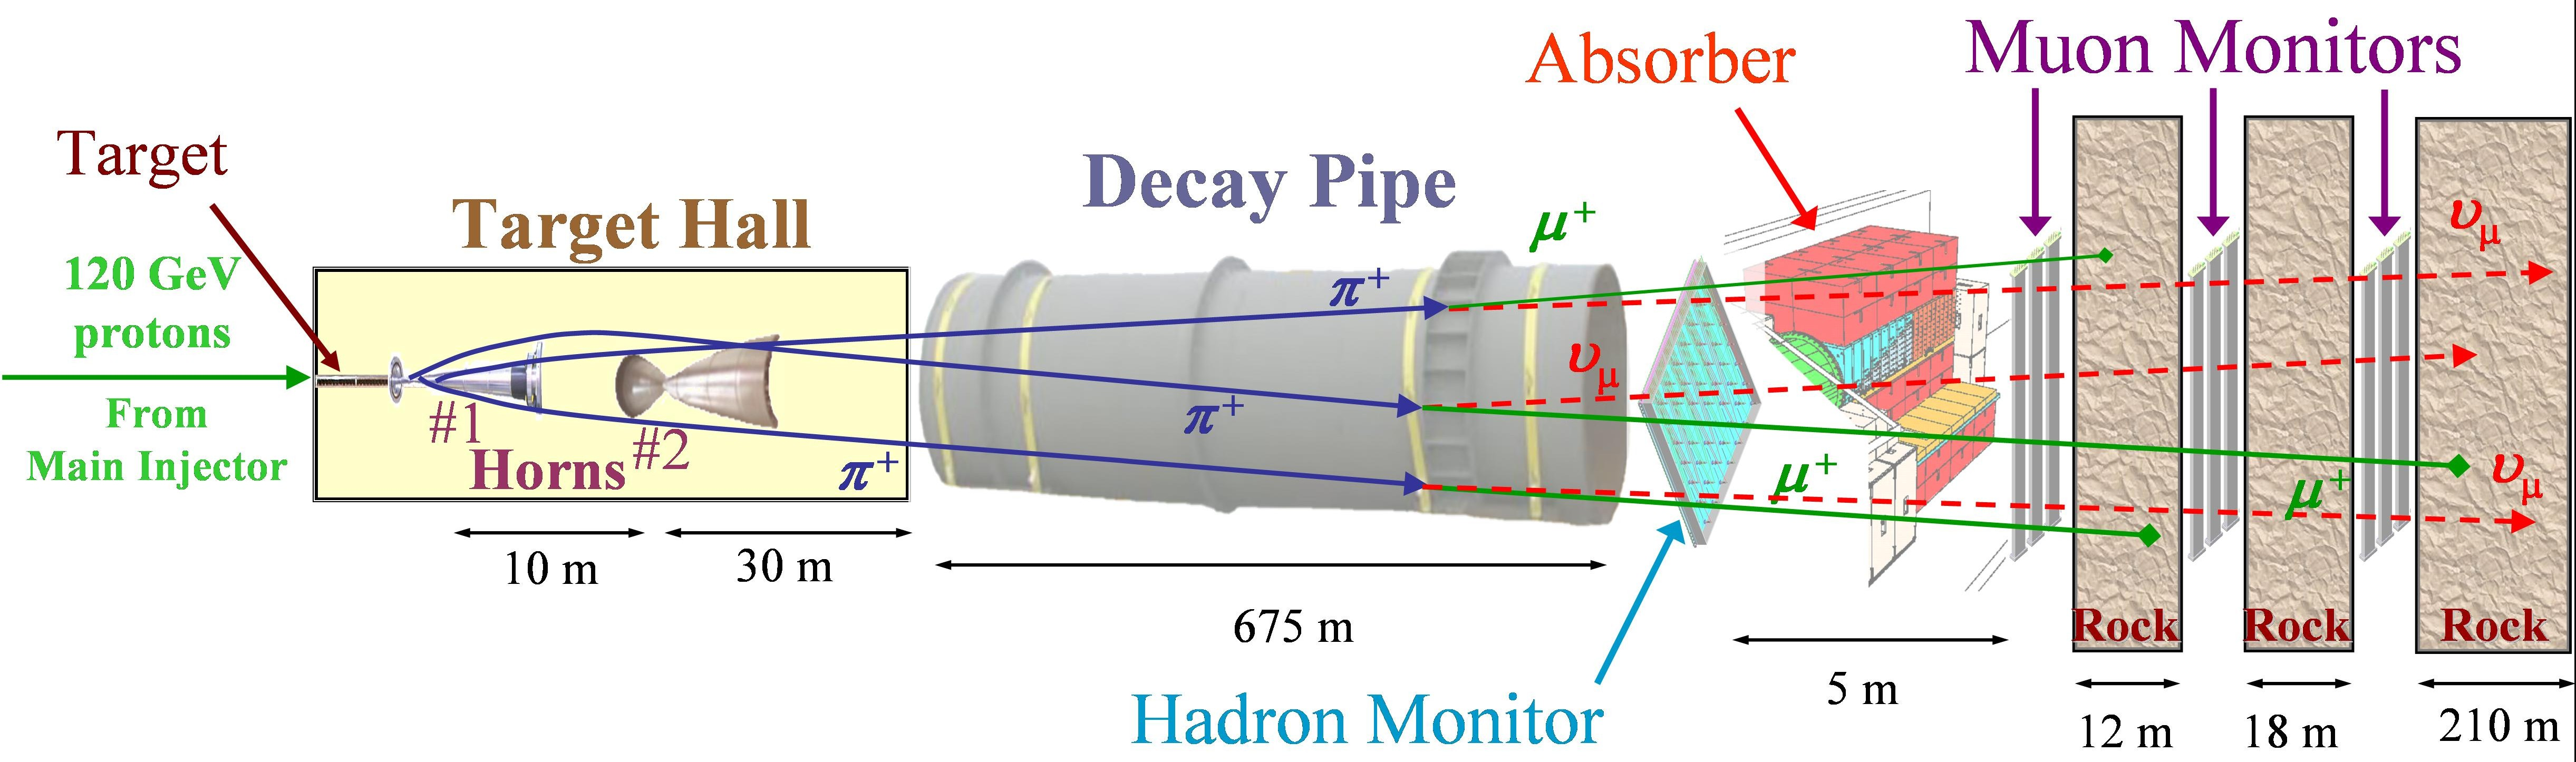
\includegraphics[width=\textwidth]{Plots/NOvAExperiment/BeamlineAlternative.jpg}
\caption[The schematic of the NuMI beam facility]{
The \acrshort{NuMI} neutrino beam starts on the left hand side with protons from the \acrshort{MI} impinged on a graphite target producing mainly pions and kaons. These are then focused and charge-selected by two focusing horns, after which they decay inside the decay pipe into a high-purity $\nu_\mu$, or $\overline{\nu}\mu$ beam. The residual hadrons are stopped and monitored in the hadron absorber and the remaining muons are recorded with muon monitors and absorbed inside the rock. Figure from \cite{NuMI.pdf}.
%The schematic of the NuMI beam facility. The beam travels from left to right. The individual components shown are not to scale. Protons originate as $H^-$ ions, which are converted into protons in the Booster, sent to the main injector, where they are finally accelerated to $120\,\si{\giga\electronvolt}$, bent downward by $58\,\si{\milli\radian}$ and transported $350\,\si{\meter}$ to the $1.2\,\si{\meter}$ long NuMI target. The protons are incident on the graphite target and the produced hadrons are focused by two magnetic horns, located in about $40\,\si{\meter}$ long target hall, with about $19\,\si{\meter}$ separation between the two horns. Hadrons then enter a $675\,\si{\meter}$ long decay pipe made of steel, with $2\,\si{\meter}$ diameter, which serves as vacuum or low density environment for the mesons to propagate and decay into tertiary mesons, charged leptons and neutrinos. A hadron monitor is located at the end of the decay volume just in front of the $5\,\si{\meter}$ thick aluminium, steel and concrete absorber to record the profile of the residual hadrons. Of the particles interacting in the absorber, the principal component (approximately $80\%$) is the proton beam that has not interacted. The remainder are mainly mesons which have not decayed in the pipe or secondary protons. The absorber not only stops most of the particles still remaining in the beam but also acts as a shield against radiation. Muons and neutrinos deposit little or no energy in the absorber and continue into unexcavated rock with three muon monitors allowing measurement of the residual muon flux. The $240\,\si{\meter}$ of rock following the absorber stops the muons remaining in the beam but allows the neutrinos to pass\cite{numi}. 
}
\label{fig:NOvANuMI}
\end{figure}

The proton beam passes through a collimating baffle before hitting a $\sim\unit[1.2]{m}$-long (equal to about two interaction lengths) graphite target \cite{LEOFluxPredictionAtNuMI.pdf}, producing hadrons, predominantly pions and kaons \cite{NuMI.pdf}. These are then focused and selected by two parabolic magnetic "horns". The focused hadrons pass through a $\unit[675]{m}$-long decay pipe filled with helium to create a low density environment for hadrons to propagate and decay in flight into either neutrinos or antineutrinos. High energy hadrons that do not decay in the decay pipe are absorbed within a massive aluminium, steel, and concrete hadron absorber and monitored with a hadron monitor. The leftover muons are ranged out in dolomite rock after the absorber and monitored using three muon monitors. The hadron and all the muon monitors are ionization chambers, used to monitor the quality, location and relative intensity of the beam.

Using a positive current inside the horns focuses positively charged particles, which then decay into neutrinos, and removes negatively charged particles. Reversing the horn current focuses negatively charged particles, which decay into antineutrinos, and defocuses positively charged particles. The neutrino mode is therefore called \gls{FHC} and the antineutrino mode is called \gls{RHC}. The composition of the neutrino beam for both these modes at the \gls{NOvA} \gls{ND}, shown as a rate of \gls{CC} events, is presented in Fig.~\ref{fig:NOvABeamComponents}, displaying the very high purity $\nu_\mu$ component in the \gls{FHC} beam, and the high purity $\overline{\nu}_\mu$ component in the \gls{RHC} mode \cite{NuMI.pdf}.

\begin{figure}[!htb]  
  \centering
  \includegraphics*[width=.495\textwidth]{Plots/NOvAExperiment/NuMIBeamComponentsCCEvtsFHC.pdf}
  \noindent\centering
  \includegraphics*[width=.495\textwidth]{Plots/NOvAExperiment/NuMIBeamComponentsCCEvtsRHC.pdf}
  \caption[NuMI neutrino beam components in the NOvA near detector]{The \acrshort{CC} event rates for different neutrino flavours, as measured at the \acrshort{NOvA} \acrshort{ND} in the \acrshort{FHC} regime shown on the left, or the \acrshort{RHC} regime on the right. The contribution of neutrino flavours to the event rates is also displayed, showing the high purity of the neutrino beam for \acrshort{NOvA}. Figure from internal \acrshort{NOvA} repository.}
 \label{fig:NOvABeamComponents}
\end{figure}

The resulting neutrino beam energy distribution is peaked at $\sim\unit[7]{GeV}$ with a wide energy band. However, thanks to the kinematics of the dominant pion decay, by placing \gls{NOvA} detector $\unit[14.6]{mrad}$ ($\approx\unit[0.8]{\degree}$) off the main \gls{NuMI} beam axis, we achieve a narrow band neutrino flux peaked at $\unit[1.8]{GeV}$ \cite{NOvAResults2021.pdf,NOvATechreport.pdf}, as can be seen in Fig.~\ref{fig:NOvAOffAxis}. Using an off-axis neutrino flux increases the neutrino beam around $\unit[2]{GeV}$ about 5-fold compared to the on-axis flux and narrow-band peak enhances background rejection for the $\nu_e$ appearance analysis \cite{NOvATechreport.pdf}.

%Protons originate as $\textsc{H}^-$ ions, accelerated by the Linac to $\unit[400]{MeV}$, converted to protons and further accelerated to $\unit[8]{GeV}$ in the Booster, to be passed to the Main Injector which finally accelerates them to $\unit[120]{GeV}$ . Protons are then extracted, bent down to point towards the MINOS/NOvA Far Detector, and transported to the NuMI target \cite{NuMI.pdf}. The current beam power is $\sim\unit[700]{kW}$ with a plan \cite{PIP2.pdf} of reaching more than $\unit[1]{MW}$ beam power in the future upgrades.
%The NuMI target is a graphite fin, $\unit[7.4]{mm}$ wide, $\unit[63]{mm}$ tall and $\approx\unit[120]{cm}$ long (along the beam direction)\footnote{Previous target proportion were $\unit[6.4]{mm}$ W, $\unit[15]{mm}$ H and $\unit[95.38]{cm}$ L used in low energy design (see lower) \cite{NuMI.pdf}.} \cite{LEOFluxPredictionAtNuMI.pdf}. Protons interact in the target producing hadrons, predominantly pions and kaons \cite{NuMI.pdf}.

%The off-axis location means that both NOvA detectors are sited $14.6\,\si{\milli\radian}$ off the NuMI beam axis, in contrast to the MINOS Far Detector. This is because at around $14\,\si{\milli\radian}$, the energy of the neutrino does not have a strong dependence on the energy of the parent pion (fig. \ref{angleoff}), and also at this angle, the medium energy beam produces a narrow energy beam with approximately five times more neutrinos at $2\,\si{\giga\electronvolt}$ (fig. \ref{off-axis}), which is well-matched to the oscillation maximum expected to be at $1.6\,\si{\giga\electronvolt}$, thus maximizing the experiment’s neutrino oscillation sensitivity. In addition to the increased flux, the narrowness of the off-axis spectra enhances background rejection.\cite{techreport}

\begin{figure}[!htb]  
  \centering
  \includegraphics*[width=.48\textwidth]{Plots/NOvAExperiment/PionOffAxis.pdf}
  \noindent\centering
  \includegraphics*[width=.51\textwidth]{Plots/NOvAExperiment/OffAxisFluxPionEmbedded.pdf}
  \caption[The NOvA off-axis beam concept]{(Left) Dependence of the neutrino energy on the parent pion's energy and (right) neutrino energy distribution for an on-axis beam and three different off-axis beam designs. The case for \acrshort{NOvA} is shown here in red and results in a narrow neutrino energy distribution around $\unit[2]{GeV}$, with limited dependence on the parent pion's energy. Figure from \cite{NOvATechreport.pdf}}
 \label{fig:NOvAOffAxis}
\end{figure}

\section{The NOvA Detectors}\label{sec:NOvADetectors}

The two main \gls{NOvA} detectors are the \gls{ND}, located in \gls{Fermilab} $\sim\unit[1]{km}$ from the \gls{NuMI} target and $\sim\unit[100]{m}$ under ground, and the \gls{FD}, located $\sim\unit[810]{km}$ from \gls{Fermilab} at Ash River in north Minnesota, partially underground with a rock overburden \cite{NOvATechreport.pdf}. \gls{NOvA} also operated a detector prototype called \gls{NDOS} used for early research and development of detector components and analysis \cite{NOvAStatusAndOutlook.pdf}. Additionally, \gls{NOvA} operated a \gls{TB} detector, described in detail in Sec.~\ref{sec:TBDetector}. The scale of \gls{ND} and \gls{FD} is shown in Fig.~\ref{fig:NOvADetectors}.

%The FD has an approximately 130kHz of cosmics

\begin{figure}[ht]
\centering
%is pdf-a
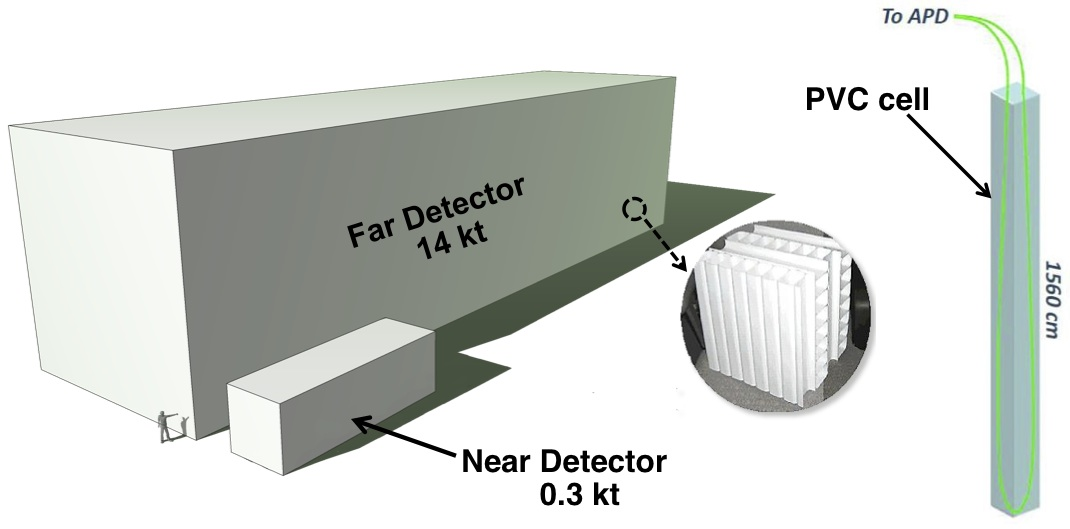
\includegraphics[width=1\textwidth]{Plots/NOvAExperiment/NOvADetectors.png}
\caption[NOvA detectors]{Schematic description of scale and composition of the \acrshort{NOvA} detectors. The inset shows a photo of the orthogonal planes made out of \acrshort{PVC} cells. An example of a \acrshort{FD} cell containing liquid scintillator and a looped \acrshort{WLS} fibre attached to an \acrshort{APD} is shown on the right \cite{NeutrinoDetectorsForOscExp.pdf}.}
\label{fig:NOvADetectors}
\end{figure}

All \gls{NOvA} detectors are highly segmented, highly active, functionally identical tracking calorimeters made up of \gls{PVC} cells filled with liquid scintillator. Each cell is a long rectangular cuboid with depth of $\unit[5.9]{cm}$ and width of $\unit[3.8]{cm}$ (with some variations), with cell length extending to the full width/height of each detector, which is $\sim\unit[4.1]{m}$ for the \gls{ND} and $\sim\unit[15.6]{m}$ for the \gls{FD} \cite{NOvATechreport.pdf}. An example of a \gls{FD} cell is shown on the right of Fig.~\ref{fig:NOvADetectors}.

Cells are connected side-by-side into a 16 cell-wide extrusions with $\unit[3.3]{mm}$-wide walls between cells and $\unit[4.9]{mm}$-wide walls on the outsides of the extrusions. The first and last cell of each extrusion are $\sim\unit[3]{mm}$ narrower than the rest of the cells. Two extrusions are connected side-by-side to form a 32 cell-wide module, with each module having a separate readout (see Sec.~\ref{sec:DAQ}). In the \gls{FD}, 12 modules are connected side-by-side to form one plane of the detector. In the \gls{ND} only 3 modules make up a plane. Planes are positioned one after another, alternating between vertical and horizontal orientation, and grouped into diblocks, each containing 64 planes. The \gls{FD} contains 14 diblocks, totalling 896 planes, whereas the \gls{ND} contains 3 diblocks totalling 192 planes. However, the \gls{ND} also consists of a Muon Catcher region, positioned right after the active region, consisting of 22 planes of the normal \gls{NOvA} detector design, 2 modules high and 3 modules wide, sandwiched with 10 steel plates to help range out muons mainly from the $\nu_\mu$ charged current interactions~\cite{NOvAStatusAndOutlook.pdf,NOvATechreport.pdf}.

\todo{Describe the coordinate system in NOvA}

Each cell is filled with a liquid scintillator consisting of mineral oil with $4.1\%$ pseudocumene as the scintillant \cite{NOvAScintillators.pdf}. Each cell contains a single wavelength shifting fibre with double the length of the cell, looping at one end and connecting to the readout at the other. As light travels through the fibre, it is attenuated by about a fraction of ten for the \gls{FD} cells \todo{Figure out what is the correct statement here}. The \gls{PVC} walls of the detector cells are loaded with highly reflective titanium dioxide, with light typically bouncing off the \gls{PVC} walls about 8 times before being captured by the fibre \cite{NOvATechreport.pdf}. 

The final dimensions of the \gls{FD} are $\unit[15.6]{m}\times\unit[15.6]{m}\times\unit[60]{m}$ with a total mass of $\unit[14]{kT}$ and for the \gls{ND} the dimensions are $\unit[3.8]{m}\times\unit[3.8]{m}\times\unit[12.8]{m}$ with a mass of about $\unit[0.3]{kT}$ \cite{NOvAHalfTimeOverview2022.pdf}. The active volume, consisting only of the liquid scintillator without the \gls{PVC} structure, makes up about $70\%$ of the total detector volume \cite{NOvATechreport.pdf}.

The \gls{NOvA} detectors are specifically designed for electromagnetic shower identification, with a radiation length of $\unit[38]{cm}$, which amounts to $\sim 7$ planes for particles travelling perpendicular to the detector planes \cite{NOvAStatusAndOutlook.pdf}. This is particularly useful to distinguish electrons and $\pi^0$s.

\todo{Talk here or in the next section about minimum electron energy to be recorded by NOvA detector and electronics. Maybe in all sections including reconstruction to tie them together}
%The MIP energy loss for electrons (similarly to muons) can be found with a similar method as used in the AbsCal\_technote\_1stAna in TestBeam (page 2)

\section{Readout and Data Acquisition}\label{sec:DAQ}

The signal from the \gls{WLS} fibres is read out by an \gls{APD}, converting the scintillation light into electrical signal, with a high quantum efficiency of $\sim 85\%$ and a gain of $100$ \cite{NOvATechreport.pdf}. An example \gls{APD} is shown in Fig.~\ref{fig:NOvAAPD}. Both ends of each fibre are connected to one of the 32 pixels on the \gls{APD}, with each \gls{APD} reading out signal from one module. To maximise the signal to noise ratio, the \gls{APD}s are cooled to $\unit[-15]{\degree C}$ by a thermoelectric cooler, with heat carried away by a water cooling system.

The combination of the \gls{APD} quantum efficiency and the light yield, determined by the \gls{PVC} reflectivity and the scintillator's and \gls{WLS} fibre's response, result in a signal requirement of at least 20 photoelectrons in response to minimum ionizing radiation at the far end of the \gls{FD} cell.

%TDR-12.2.1:"NOvA readout electronics requires, at minimum, a 20 photoelectron signal in response to minimum ionizing radiation at the far-end of a 15.5 m NOvA cell as discussed in Chapter 6. The signal strength is due to the APD quantum efficiency and the light yield in response to ionizing radiation. The light yield, in turn, is due to a combination of the PVC reflectivity, the scintillator and wavelength-shifting fiber responses."

%For some reason the TDR I have downloaded doesn't have the full chapter 14. Full TDR can be found in docdb:2678 chapter by chapter.

\begin{figure}[!htb]  
  \centering
  \includegraphics*[width=.495\textwidth]{Plots/NOvAExperiment/NOvAAPDMountedWithLabels.jpg}
  \noindent\centering
  \includegraphics*[width=.495\textwidth]{Plots/NOvAExperiment/NOvAAPDBottomWithLabels.jpg}
  \caption[NOvA Avalanche Photo Diods]{The modules with \acrshort{APD}s for \acrshort{NOvA} mounted on top of the detector on the left picture, and shown from the bottom on the right. The individual components of the module are described. The left picture shows a disconnected ribbon cable and ground cable, which are normally connected to the front end board.}
 \label{fig:NOvAAPD}
\end{figure}

Each \gls{APD} is connected to a single \gls{FEB}, shown in Fig.~\ref{fig:NOvAFEB}. The \gls{FEB} amplifies and integrates the \gls{APD} signal, determines its amplitude and arrival time, before passing it to the \gls{DAQ} system. On the \gls{FEB} the \gls{APD} signal is first passed to a custom \gls{NOvA} \gls{ASIC}, which is design to maximize the detector sensitivity to small signals. \gls{ASIC}s amplify, shape and combine the signal, before sending it to an \gls{ADC}. The combined noise from the \gls{APD} and the amplifier is equivalent to about 4 \gls{PE}s, which, compared to an average photoelectron yield from the far end of the \gls{FD} cell of 30, results in a good signal and noise separation \cite{NOvATechreport.pdf}. The digitized data from an \gls{ADC} is sent to a \gls{FPGA}, which extracts the time and amplitude of the \gls{ADC} signals, while subtracting noise based on a settable threshold. The \gls{FPGA}s employ multiple correlated sampling methods to reduce noise and improve time resolution of the signal \cite{NOvADAQ.pdf}.

\todo{Find out what is the pedestal/threshold that's being subtracted}

\begin{figure}[!htb]  
  \centering
  \includegraphics*[width=\textwidth]{Plots/NOvAExperiment/NOvAFEBWithLabels.jpg}
  \caption[NOvA Front End Board]{An example of a \acrshort{NOvA} \acrshort{FEB} with individual components labelled.}
 \label{fig:NOvAFEB}
\end{figure}

%TDR:Major components are the carrier board connector location at the left, which brings the APD signals to the NOvA ASIC, which performs integration, shaping, and multiplexing. The chip immediately to the right is the ADC to digitize the signals, and FPGA for control, signal processing, and communication. Data from the ADC is sent to an FPGA where multiple correlated sampling is used to remove low frequency noise. This type of Digital Signal Processing (DSP) also reduces the noise level and increases the time resolution.

All of the \gls{NOvA} front end electronics (\gls{APD}s and \gls{FEB}s) are operated in a continuous readout mode, without requiring any external triggers \cite{NOvATechreport.pdf}. Due to higher detector activity during beam spills, the \gls{ND} \gls{FEB}s work at a higher frequency of $\unit[8]{MHz}$, whereas the \gls{FD} \gls{FEB}s suffice with $\unit[2]{MHz}$ sampling frequency \cite{NOvADAQ.pdf}.

Data from up to 64 \gls{FEB}s are concentrated in a \gls{DCM}, which concatenates and packages the data into $\unit[5]{ms}$ time slices, before sending it to the buffer nodes. \gls{DCM}s are also connected to the timing system and pass a single unified timing measurement to the \gls{FEB}s to maintain synchronization across the detector~\cite{NOvADAQ.pdf}.
%The timing information is calibration off-line to account for differences between fibre and cable distances and to achieve a superb timing resolution \cite{NinerThesis} - I don't think I need to talk about the timing calibration here tbh. The NOvA calibration process technically also involves \textbf{timing calibration}, which corrects for the time differences of the signal to be processed \cite{NinerThesis}.

The buffer nodes cache the data for at least 20 seconds while receiving information from the trigger system. Each trigger uses a time window based either on the time of the \gls{NuMI} beam spill, on a periodic interval for readout of comic events for detector calibration and monitoring, or on a time of activity-based data-driven trigger \cite{NOvADAQ.pdf}. Data that fall within any of the trigger windows are sent to a data logger system, where they are merged to form events, before being written to files for offline processing, or sent to an online monitoring system.

%Data for calibration and non-beam physics channels is collected and a variety of data-driven triggers using real-time reconstruction algorithms run on data stored in an online buffer farm at each detector [26].  Beam events are collected in both detectors using a 550 μs time window centered on the 10 μs beam spill window, triggered by a signal derived from the accelerator controls system. The wide time window of data collection compared to the beam spill is used to sample cosmic-ray activity and noise under the precise detector conditions that apply to the beam data. [NOvAHalfTimeOverview2022.pdf]

%Maybe I should write here what is the event rate?

%Maybe write about what information do we have about each event at this stage: timing, peak ADC, cell, plane, run, subrun. Grouped into triggered windows?
% "the time, location, and pulseheight of those signals are recorded as a hit" [NOvAHalfTimeOverview2022.pdf]

\note{Maybe talk about data quality as well? Probably should since I want to talk about good runs and bad channels in the TB calib chapter}

\section{Simulation}\label{sec:NOvASimulation}

\note{Should I divide the simulation into the individual stages? I had it like that originally, but for example the simulation of cosmics is only very short and not sure what section would I put it under}

To extract neutrino oscillation parameters, or to test a hypothesis, \gls{NOvA} uses a series of simulations to make predictions according to various physical models \cite{NOvASimulationOld-Fluka.pdf}.
%To simulation the expected signal from the NOvA detectors,
%To get a prediction of any possible signal events or their background in the NOvA detectors,
% we use a series of simulations, tuned or corrected by both internal and external measurements to better match the current state of the art knowledge \cite{NOvASimulationOld-Fluka.pdf}.
The simulation chain can be divided into four parts: simulation of the neutrino beam, simulation of neutrino interactions within the \gls{NOvA} detectors, simulation of cosmic particles interacting in the \gls{NOvA} detector and simulation of the detector response.

To simulate the neutrino beam, \gls{NOvA} uses the \texttt{GEANT4} v9.2.p03~\cite{GEANT4.pdf} based \gls{MC} simulation with a detailed model of the \gls{NuMI} beamline \cite{ZPavlovicThesisG4NuMI_2008.pdf}, as it was described in Sec.~\ref{sec:NOvASimulation}. The simulation starts with \gls{MI} protons interacting within the long carbon target and producing hadrons, mainly $\pi, K$ and $p$, followed by transport and possible further interaction of these hadrons within the focusing system, until finally ending with hadron decays producing the neutrino beam.

To account for the imprecise theoretical models used in GEANT4, we use the \gls{PPFX} to incorporate external measurements of yields and cross sections of hadron production inside the target and other \gls{NuMI} materials into the prediction~\cite{NuMIFlux.pdf}. The current version of \gls{PPFX} is limited by the results available during its creation and only corrects the most frequent interactions while assigning large systematics uncertainties to the rest (see Sec.~\ref{sec:NOvASystematics}). For the most common $\pi$ production, \gls{PPFX} uses the NA49 measurements \cite{NA49:Inclusive_production_of_charged_pions.pdf} of $\unit[158]{GeV/c}$ protons interacting on a thin (few percent of interaction length) carbon target, with a few data point from Barton et al~\cite{BartonHadProd1983.pdf} to expand the kinematic coverage. These then have to be scaled to the $\unit[20-120]{GeV/c}$ incident proton energies seen in \gls{NOvA} using the FLUKA \cite{FLUKA_01,FLUKA_02} \gls{MC} generator. For the $K$ production from $p+C$ interaction, important for higher neutrino energies and electron neutrinos, \gls{PPFX} uses the NA49 $K$ data \cite{NA49DataKaons.pdf} together with the NA49 $\pi$ data \cite{NA49:Inclusive_production_of_charged_pions.pdf} multiplied by the $K/\pi$ ratios of yields on thin carbon target from the MIPP experiment \cite{pionToKaonIn_pC.pdf}. Lastly, for the nucleon production, \gls{PPFX} uses the NA49 data on quasi elastic interactions \cite{NA49pc-proton2013.pdf}. All the other interactions inside \gls{NuMI}, such as interaction in non-carbon targets, or interactions with hadrons other than protons, are either extrapolated from the previously mentioned measurements, or are not corrected for and a significant systematic uncertainty is assigned to them \cite{NuMIFlux.pdf}.

There's two new experiments that measured the production and interaction of hadrons on various targets and incident energies, specifically designed to improve the prediction of neutrino beams. I worked on implementing data from the NA61 experiment on hadron production from $p+C$ interaction on a thin carbon target at $\unit[31]{GeV/c}$~\cite{2015_hadron_prod_pC_2009data.pdf}, motivated by possible reduction in the $K$ production systematic uncertainty. This work is still ongoing and will be implemented into \gls{PPFX} and \gls{NOvA} together with the rest of the NA61 measurement. The most impactful ones will be the measurement of hadron production from $p+C$ interaction on a thin carbon target at $\unit[120]{GeV/c}$ \cite{NA61_hadprodFrompC_120GeV_2023.pdf} (no energy scaling required), measurements of $p+C$ and $p+Be$ at different incident energies \cite{2019_NA61_ProdAndInelXSec_protonOnDiffTargets60And120GeV._results.pdf}, $\pi+C$ and $\pi+Be$ measurements at $\unit[60]{GeV/c}$~\cite{2019_had_prod_at_Pi_on_C_and_Be.pdf}, resonance production measurements from $\unit[120]{GeV/C}$ $p+C$ \cite{NA61_ResonanceProdFrompC_120GeV_2023.pdf}, and probably the most impactful one, the yet unpublished measurement of hadron production yield on a \gls{NOvA}-era \gls{NuMI} replica target at $\unit[120]{GeV/c}$ \cite{ThickTargetLimit.pdf}. NA61 also measured the hadron production yield for the \gls{T2K} experiment's replica target \cite{2019_hadron_yields_T2K_replica.pdf}, which significantly reduced the neutrino flux systematic uncertainty for the \gls{T2K} measurements \cite{ThickTargetLimit.pdf}. The second experiment is EMPHATIC~\cite{EMPHATICProposal2019.pdf}, which is currently analysing their data on a broad range of hadron production measurements, mainly the secondary and tertiary interactions of various projectiles with a wide range of incident energies and thin target materials, complementary to the NA61 measurements.

%From NOvAResults2021.pdf: The neutrino flux delivered to the detectors is calculated using GEANT4-based simulations of particle production and transport through the beamline components [NuMI.pdf,GEANT4.pdf] reweighted to incorporate external measurements using the package to predict the flux (PPFX) [NuMIFlux.pdf,30–48].

%From NOvAResultsCombinedNuAnu2019.pdf: The flux of neutrinos delivered to the detectors is calculated using a simulation of the production and transport of particles through the beamline components [22,25] reweighted to incorporate external measurements [26–45].

%From NOvAHalfTimeOverview2022.pdf: Neutrino interactions in NOvA are simulated with a chain of software packages. The neutrino flux is modeled using G4NuMI, a geant based description of the NuMI beam line [Z. Pavlovic thesis]. The raw flux from G4NuMI is then modified using the PPFX package to better match the products of the interactions in the extended target to the world’s hadron production data [NuMIFlux.pdf].

%%%%%%%%%%%%%%%%%%%%%%%%%%%%%%%%%%%%%%%%%%%%%%%%%%%%%%%%%%%%%%%%%%%%%%%%%%%%%%%
%%%% Master's thesis on flux simulation
\iffalse
There are often multiple interactions within the target and in the materials downstream of it and since the hadron production process is governed by non-perturbative QCD and occurs in the nucleus, highly accurate theoretical predictions are not possible \cite{NuMIFlux.pdf,LEOFluxPredictionAtNuMI.pdf}. NOvA therefore tunes and corrects possible mismodeling of the model using external data in a package developed for MINERvA experiment called Package to Predict the Flux (PPFX) \cite{LEOFluxPredictionAtNuMI.pdf}.

%...Those models are not necessarily accurate but can be tuned or benchmarked by comparing their predictions to measurements of hadron production. Recent measurements of pion production on a thick (two interaction length) carbon target have been released by MIPP [4], and measurements of pion production on a thin (few per cent interaction length) carbon target are available from NA49 [5]. In addition, there are several other hadron production measurements on various materials, using both proton and pion beams, that can be used to constrain a neutrino beamline simulation.[NuMIFlux.pdf]

%Roughly 85% of the interactions that produce particles that lead to muon neutrinos passing through MINERvA are from protons interacting on carbon. Other relevant materials are aluminum (horns), iron (decay pipe walls), helium (decay pipe gas), and air (target hall). Interactions of π ± , K ± and n created in the initial proton interaction, or subsequent interactions, are subdominant but non-negligible. When protons collide with carbon, the interactions can produce pions, kaons, neutrons, strange baryons, and lower energy protons. These particles, if they do not decay first, can interact either in the target or in other downstream material to create tertiary particles that can also decay into neutrinos. \cite{NuMIFlux.pdf}

PPFX is used to correct each interaction of neutrino's ancestry chain by weighting it with a factor computed from external experimental measurements of yields or invariant differential cross-sections \cite{LEOFluxPredictionAtNuMI.pdf}

The kinematic values of the initial particles (like the initial $\unit[120]{GeV}$ proton interacting on carbon in NuMI) are not always the same between the measured interaction and the required values. To solve this we use the \textit{Feynman-x} ($x_{F}$) scaling variable. Feynman speculated \cite{feynman1969.pdf} that expressing the cross-sections of inclusive high energy hadronic collisions in terms of $x_{F}$ would make the cross-section scaling energy independent \cite{LEOFluxPredictionAtNuMI.pdf}.
%$c_i$ is the \textit{central value} of the weight

There are two main experiments whose results are used in the PPFX. NA49 \cite{NA49:Inclusive_production_of_charged_pions.pdf}, which used $\unit[158]{GeV}$ protons interacting on carbon thin target, and MIPP \cite{pionToKaonIn_pC.pdf} which used protons from the Main Injector and both thin carbon target and the low energy NuMI target (thick target) \cite{PPFXTechnote2017.pdf}. Energy scaling of the external data to calculate the PPFX weight is performed by FLUKA\cite{NuMIFlux.pdf}

%%% Hadron production datasets:
%There are two major datasets available to constrain the process where protons interact on carbon and produce charged pions. One measurement, from NA49 [5], uses a thin target with an incident proton momentum of 158 GeV/c. The other measurement, from MIPP [4], uses an actual NuMI LE target and 120 GeV/c protons. These two datasets will be used to make separate “thin target” and “thick target” flux predictions by weighting each interaction leading to a neutrino going through MINERvA. We also use additional datasets to constrain kaon and nucleon production, and the absorption of particles in beamline materials. Where multiple interactions are constrained with data, the overall weight applied to the neutrino event is simply the product of the weights for each interaction.\cite{NuMIFlux.pdf}

For kaons with $x_{F}<0.2$ PPFX uses weights based on NA49 measurements\cite{NA49DataKaons.pdf} and for kaons with $0.2<x_{F}<0.5$ PPFX uses the $K/\pi$ yield ratio from the MIPP thin target measurements\cite{pionToKaonIn_pC.pdf} multiplied by NA49 thin target yields.
\fi
%%% End of master's on flux simulation
%%%%%%%%%%%%%%%%%%%%%%%%%%%%%%%%%%%%%%%%%%%%%%%%%%%%%%%%%%%%%%%%%%%%%%%%%%%%%%%

%Good description of PPFX, beam transport and the principal components is in the NOvA-T2K technote for Flux (doc-db:54582) https://nova-docdb.fnal.gov/cgi-bin/sso/ShowDocument?docid=54582

\note{The description of neutrino interactions, including QE/Res/DIS scattering and nuclear effects will probably be in the theory chapter. If not I'll add it here.}
\note{Might have to describe some of these interaction models a bit more if any of the cross section uncertainty for the magnetic moment analysis turns up to be significant}

The output of the neutrino beam simulation is passed to the simulation of neutrino interactions inside the detectors, which is done with the GENIE v3.0.6~\cite{GENIE.pdf} neutrino \gls{MC} generator. GENIE allows users to choose the particular models for different types of neutrino interactions and particle propagation within the nucleus, as well as possible tunes to external measurements. The four main interaction modes in GENIE are the \gls{QE} \gls{CC} scattering, the \gls{Res}, the \gls{DIS}, and the \gls{COHpi}. Special case of \gls{CC} interaction with two nucleons producing two holes via \gls{MEC} is also considered. Particles created in these processes are then propagated inside the nucleus according to the \gls{FSI}. All of these are set by the \gls{CMC} and \gls{NOvA} currently uses the \texttt{N1810j0000} \gls{CMC}. Additionally, \gls{NOvA} adds a tune to \gls{NOvA} $\nu_\mu$\gls{CC} data for the \gls{CC}\gls{MEC} interactions and a set of external $\pi$ interaction measurements to constrain the \gls{FSI} model. Table~\ref{tab:NuIntSimulationModels} shows the list of models and tunes for different interaction modes in \gls{NOvA} \cite{NOvAResults2021.pdf}.

\begin{table}[!ht]
\centering
%\def\arraystretch{1.4}
\caption{Models and tunes used in the NOvA simulation of neutrino interactions.}
\begin{tabular}{|l|l|l|}
\hline
Interaction & Model                  & Tune\\\hline
\gls{CC}\gls{QE} & Val\`{e}ncia \cite{ValenciaModel_NOvACCQE_2004.pdf} & External $\nu-\textsf{D}$ data \cite{NuDeuteriumScattering_NOvACCQETune_2016.pdf}\\
\gls{CC}\gls{MEC} & Val\`{e}ncia \cite{ValenciaModel_NOvACCQEMEC_2011.pdf,ValenciaModel_NOvAMEC_2013.pdf} & \gls{NOvA} $\nu_\mu$\gls{CC} data\\
\gls{Res} \& \gls{COHpi} & Berger-Sehgal \cite{BergerSehgal_ResonancePionProd_2007.pdf,BergerSehgalModel_CohPionProd_2009.pdf}          & External $\nu-A$ data\\
\gls{DIS} & Bodek-Yang \cite{BodekYangModel_NOvADIS_2003.pdf,HadronizationModelForNuDIS_NOvADIS_1988.pdf}            & External $\nu-A$ data\\
\gls{FSI} & Semi-classical cascade \cite{FSIModel_hNSemiClassicalCascade_1988.pdf} & External $\pi-^{12}\textsf{C}$ data\\\hline
\end{tabular}
\label{tab:NuIntSimulationModels}
\end{table}

%NOvANuMuCCPi0XSecMeasurement2023.pdf: Neutrino interactions are simulated with GENIE [17] v2.10.2. The GENIE simulation generates interactions via its four default production processes: quasielastic scattering, resonant baryon production, deep-inelastic scattering, and coherent pion production. Particles created via these primary processes are subsequently propagated though the nuclear medium using GENIE’s hA effective cascade FSI model [18,19].

% Describe that GENIE is highly costumizable and you can set up any generators you like. Ideally describe what parts are purely theoretical and what parts are tuned to external data. Also mention that NOvA is doing an internal tune to some of the parameters.

%From NOvAResults2021.pdf: Neutrino interactions are simulated using a custom model configuration of GENIE 3.0.6 [49,50] tuned to external and NOvA ND data.
%In this configuration, charged-current (CC) quasielastic (QE) scattering is simulated using the model of Nieves et al. [53], which includes the effects of long-range nucleon correlations calculated according to the random phase approximation (RPA) [53–55]. The CCQE axial vector form factor is a z-expansion parametrization tuned to neutrino-deuterium scattering data [56].
%CC interactions with two nucleons producing two holes (2p2h) are given by the IFIC València model [57,58]. The initial nuclear state is represented by a local Fermi gas in both the QE and 2p2h models, and by a global relativistic Fermi gas for all other processes.
%Baryon resonance (RES) and coherent pion production are simulated using the Berger-Sehgal models with final-state mass effects taken into account [59,60].
%Deep inelastic scattering (DIS) and nonresonant background below the DIS region are described using the Bodek-Yang model [61] with hadronization simulated by a data-driven parameterization [62] coupled to PYTHIA [63].
%Bare nucleon cross sections for RES, DIS, and nonresonant background processes are tuned by GENIE to neutrino scattering data.
%Final-state interactions (FSI) are simulated by the GENIE hN semi-classical intranuclear cascade model in which pion interaction probabilities are assigned according to Oset et al. [64] and pion-nucleon scattering data.

%The 2p2h and FSI models in this GENIE configuration are adjusted to produce a NOvA-specific neutrino interaction model tune. The 2p2h model is fit to $\nu_\mu$CC inclusive scattering data from the NOvA ND. Inspired by Gran et al. [65], this 2p2h tune enhances the base model as a function of energy and momentum transfer to the nucleus and is applied to all CC 2p2h interactions for both the neutrino and antineutrino beams. 
%The parameters governing $\pi^\pm$ and $\pi^0$ FSI are adjusted to obtain agreement with $\pi^+$ on $^{12}\textsf{C}$ scattering data [66–72].

%From NOvAResultsCombinedNuAnu2019.pdf: Neutrino interactions in the detector are simulated using GENIE [46] tuned to improve agreement with external measurements and ND data, reducing uncertainties in the extrapolation of measurements in the ND to the FD. As in Ref. [21], we set MA in the quasielastic dipole form factor to 1.04 GeV/c2 [47] and use corrections to the charged-current (CC) quasielastic cross section derived from the random phase approximation [48,49]. In this analysis, we also apply this effect to baryon resonances as a placeholder for the unknown nuclear effect that suppresses rates at a low four-momentum transfer in our and other measurements [50–53]. Additionally, we increase the rate of deep-inelastic scattering with hadronic mass W > 1.7 GeV/c2 by 10\% to match our observed counts of short track-length $\nu_\mu$CC events. We model multinucleon ejection interactions following Ref. [54] and adjust the rates in bins of energy transfer, $q_0$, and three-momentum transfer, $\left|\overrightarrow{q}\right|$, for $\nu_\mu$ and $\overline{\nu}_\mu$ separately to maximize agreement in the ND. The calculation of the $\nu_e$ and $\overline{\nu}_e$ rates uses these same models.

%From NOvAHalfTimeOverview2022.pdf: Neutrino interactions and final state interactions are modeled using the GENIE neutrino interaction generator [31]

%From master thesis: From there GENIE event generator \cite{GENIE.pdf} simulates neutrino interactions in the detector \cite{2019NOvAFHCRHCResults.pdf} and another GEANT4 simulates the detector response \cite{NOvASimulationOld-Fluka.pdf}. NOvA also tunes the cross-section model of the GENIE simulation to the ND data to reduce uncertainties in the extrapolation of measurements on the ND to the FD \cite{2019NOvAFHCRHCResults.pdf}.

Since the \gls{FD} is on the surface we also need to include a simulation of cosmic rays generated with the CRY \cite{CRY} \gls{MC} generator. The simulated cosmic muons are also used to calibrate \gls{NOvA} detectors \cite{NuMIFlux.pdf}. 

Particles that are created from neutrino interactions and cosmic rays are propagated through the \gls{NOvA} detectors using an updated version of \texttt{GEANT4} v10.4.p02~\cite{GEANT4.pdf}. The output of this simulation is the energy deposited in the scintillator, which is then passed to a custom \gls{NOvA} simulation software \cite{NuMIFlux.pdf}. The scintillation light generated by the deposited energy is parametrized using the Birks-Chou model \cite{BirksChouParametrization_1952.pdf}, which corrects for recombination in organic scintillators at high deposited energies. The normalization factors for the produced scintillation light (the light yield), as well as for the Cherenkov light, which can affect the light readout, are tuned to \gls{NOvA} cosmic data~\cite{NOvANumuCCXSexMeasurement2023.pdf}. The light collection by the \gls{WLS} fibres and its transport to the \gls{APD}s, as well as the \gls{APD} response use a parametrized simulation, which makes use of the fact that all the \gls{NOvA} cells and their readout are generally the same across the detectors \cite{NuMIFlux.pdf}. The simulation of the readout electronics is done by another custom \gls{NOvA} parametrized model, which mainly account for a random electronics noise, with output in the same format as raw data.

%NuMIFlux.pdf: While GEANT4 is capable of simulating optical photon processes, generating scintillation light and propagating it through the cell, up the fiber, and to the APD is very time consuming. Instead, we observe that the NOvA detectors are composed of many identical readout cells as shown in Fig. 6, so if we can generate templates to parameterize photon transport once, we can use them everywhere. The processes we must be able to parameterize are: the collection of scintillation photons by the fiber, the transport of light up the fiber, and the response of the APD to the captured light.

Due to the high neutrino rate in the \gls{ND}, there are neutrinos interacting in the surrounding rock creating particles that make it to the detector and act as background. To simulate these rock events we use the same simulation as for neutrino interactions inside the detector. However, since only a few particles make it into the detector, it would be very time consuming to run this simulation for every neutrino. Therefore, we create a separate simulation that includes the surrounding rock and then overlay the results into the normal \gls{NOvA} simulation chain, which doesn't include the rock, so that the rate matches the \gls{NuMI} neutrino rate \cite{NuMIFlux.pdf}.

%%% Rock simulation and overlay
%NuMIFlux.pdf: Due to the high beam intensity at the near detector, many neutrinos interact in the rock in front of the detector. Simulating these interactions requires allowing GEANT4 to propagate muons through a very large rock volume which is a slow process, and only a few of these muons will make it into our detector. To correctly account for this, we simulate many neutrino interactions with the mother volume including a large rock volume in front of the detector, and only keep those that leave energy in the detector. During normal simulation, with the mother volume only including the detector and the immediate detector hall, we overlay these rock ’singles’ at a rate determined during the generation of flux files after the GEANT4 stage.

\section{Data Processing and Event Reconstruction}\label{sec:NOvAReconstruction}
Both data and simulation events for all \gls{NOvA} detectors are passed through the same event reconstruction and particle identification algorithms. The reconstruction was specifically developed with the $\nu_e$ appearance search in mind, focusing on identifying the $\nu_e$\gls{CC} signal against the $\nu_\mu$\gls{CC} and \gls{NC} backgrounds. Each \gls{NOvA} detector has to deal with a different challenges, with multiple neutrinos interacting in the \gls{ND} during one beam spill, and a large cosmic background in the \gls{FD} \cite{NOvAReco.pdf}.

The readout from each cell from the \gls{DAQ} (see Sec.~\ref{sec:DAQ}) is called a \textit{channel} and the \gls{DAQ} output from each channel is called a \textit{raw hit}. \gls{DAQ} groups hits into $\unit[550]{\mu s}$ windows and passes them to an offline reconstruction chain~\cite{NOvAReco.pdf}. Reconstruction starts by grouping hits into \textit{slices} based on their proximity to other hits in both time and space~\cite{DBSCAN.pdf}.
\note{Maybe include rawhit to cellhit to recohit}
%[RelCal_technote_1stAna.pdf] CalHit transforms RawDigits into CellHits. This is a transformation of the channel numbering system to offline (plane/cell) coordinates, and the fine-timing fit. A RecoHit can by created from a CellHit by passing it and an estimated W position to Calibrator, or by asking one of the RecoBase objects, which calculate best-guess W positions for their constituent cells.

For events that produce hadronic and electromagnetic showers, we first identify lines through major features using a modified Hough transform~\cite{HoughTransform.pdf}. These lines representing momentum directions are then passed to the Elastic Arms algorithm~\cite{ElasticArms.pdf} to identify \textit{vertex} candidates from their intersection points. Hits are then clustered into \textit{prongs}, group of hits with a start point and a direction, using a k-means algorithm called FuzzyK \cite{FuzzyKClustering.pdf,FuzzyKFuzzyness.pdf}. Here "fuzzy" means that each hit can belong to multiple prongs. Prongs are first created separately for each view (also called 2D prongs) and then, if possible, view-matched into 3D prongs (or just prongs)~\cite{NOvAReco.pdf}. Figure~\ref{fig:NOvARecoEVD} shows an example simulated electron shower with the reconstructed vertex (red cross) and prong (red shaded area) grouping all hits that should be a part of the shower together, while removing background hits in grey.

\begin{figure}[ht]
\centering
%is pdf-a
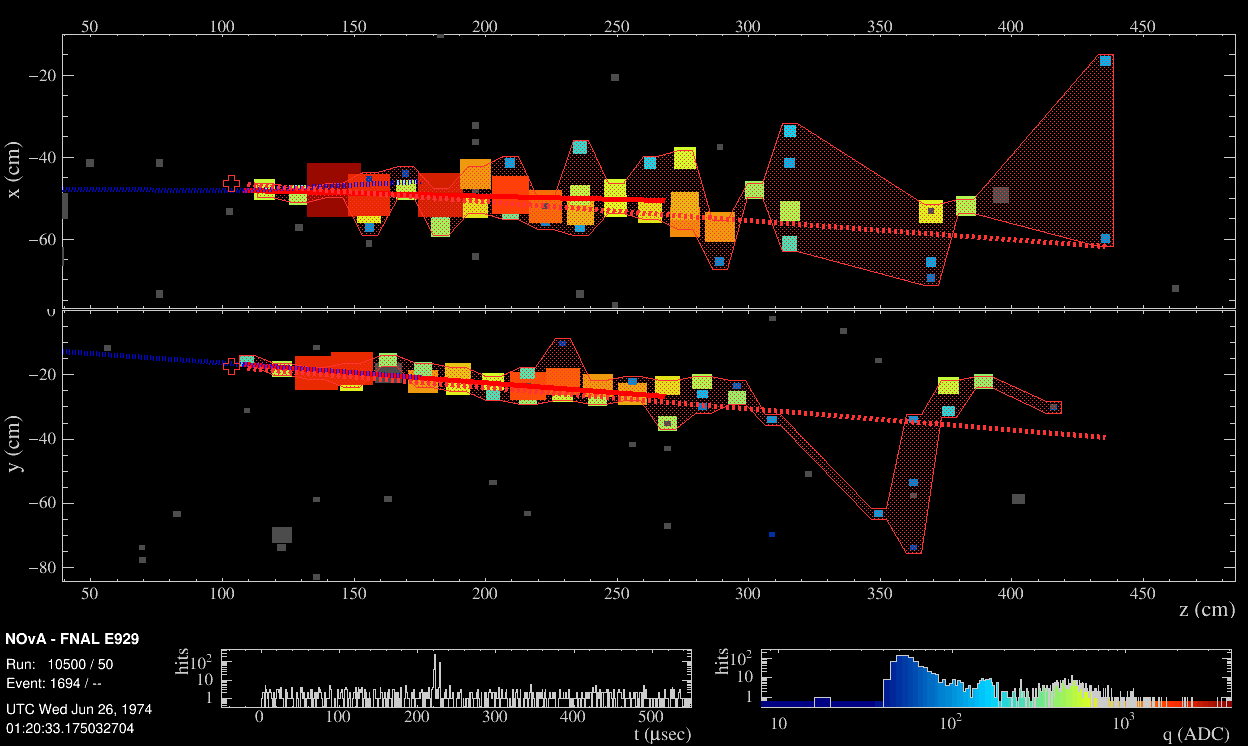
\includegraphics[width=1\textwidth]{/home/robert/Documents/School/PhD/Thesis/Plots/NOvAExperiment/ElectronRecoEVD.png}
\caption[NOvA reconstruction of a single electron]{Reconstruction of a simulated single electron event in the \acrshort{NOvA} \acrshort{ND}. The red cross is the reconstructed vertex, the shaded area shows the cluster of hits into a shower and the dotted red line shows the estimated momentum of that shower. The blue dotted line shows the true momentum of the scattering neutrino and the solid red line the true momentum of the scattered electron. Figure from internal \acrshort{NOvA} database.}
\label{fig:NOvARecoEVD}
\end{figure}

For particles that are represented by tracks rather than showers (especially muons) we take the slice hits and form the \textit{Kalman tracks} based on a Kalman filter~\cite{RaddatzNOvAThesis_KalmanTracks.pdf}. In addition to the start point and the direction, which exist also for prongs, tracks also contain information on the vector of trajectory points that make up the track and on the end point - and therefore on the track length. A parallel tracking algorithm takes in the Elastic Arms vertex and the Fuzzy-K 3D prongs and forms \gls{BPF} tracks \cite{BairdNOvAThesis_BPFTracks.pdf,BreakPointFitterBasics.pdf}, using a model of Coulomb scattering and energy loss. \gls{BPF} tracks also contain 4-momentum information based on various particle assumption, most notably muon assumption. For cosmic particles, mostly muons, we use another track reconstruction algorithm, called the window cosmic track algorithm~\cite{NOvA-doc-15977}. The window cosmic track algorithm uses a sliding 5 plane-long window, starting from the end of the detector, in which it fits a straight line to the recorded hits, before sliding the window forward and repeating the process. This way it accounts for possible Coulomb scattering of cosmic muons.

%%% PID

To identify individual particles and remove backgrounds, \gls{NOvA} uses several \gls{ML} algorithms, outputs of which are used in for \gls{PID} in various \gls{NOvA} analyses. The most common topologies for particles interacting in \gls{NOvA} detectors are shown on Fig.~\ref{fig:NOvAEventTopologies}. Muons are easily identifiable as a single long track which decays into an electron (or positron) if it stops inside the detector. Both electrons and $\pi^0$'s produce electromagnetic showers, but thanks to the low-Z composition and high granularity of the detector, there is a gap between the interaction vertex and the electromagnetic shower.

%A Kalman-like algorithm is used with a BDT based on energy loss, multiple scattering, and length parameters of a candidate track to identify muons and reconstruct their energy using track length.

\begin{figure}[ht]
\centering
%is pdf-a
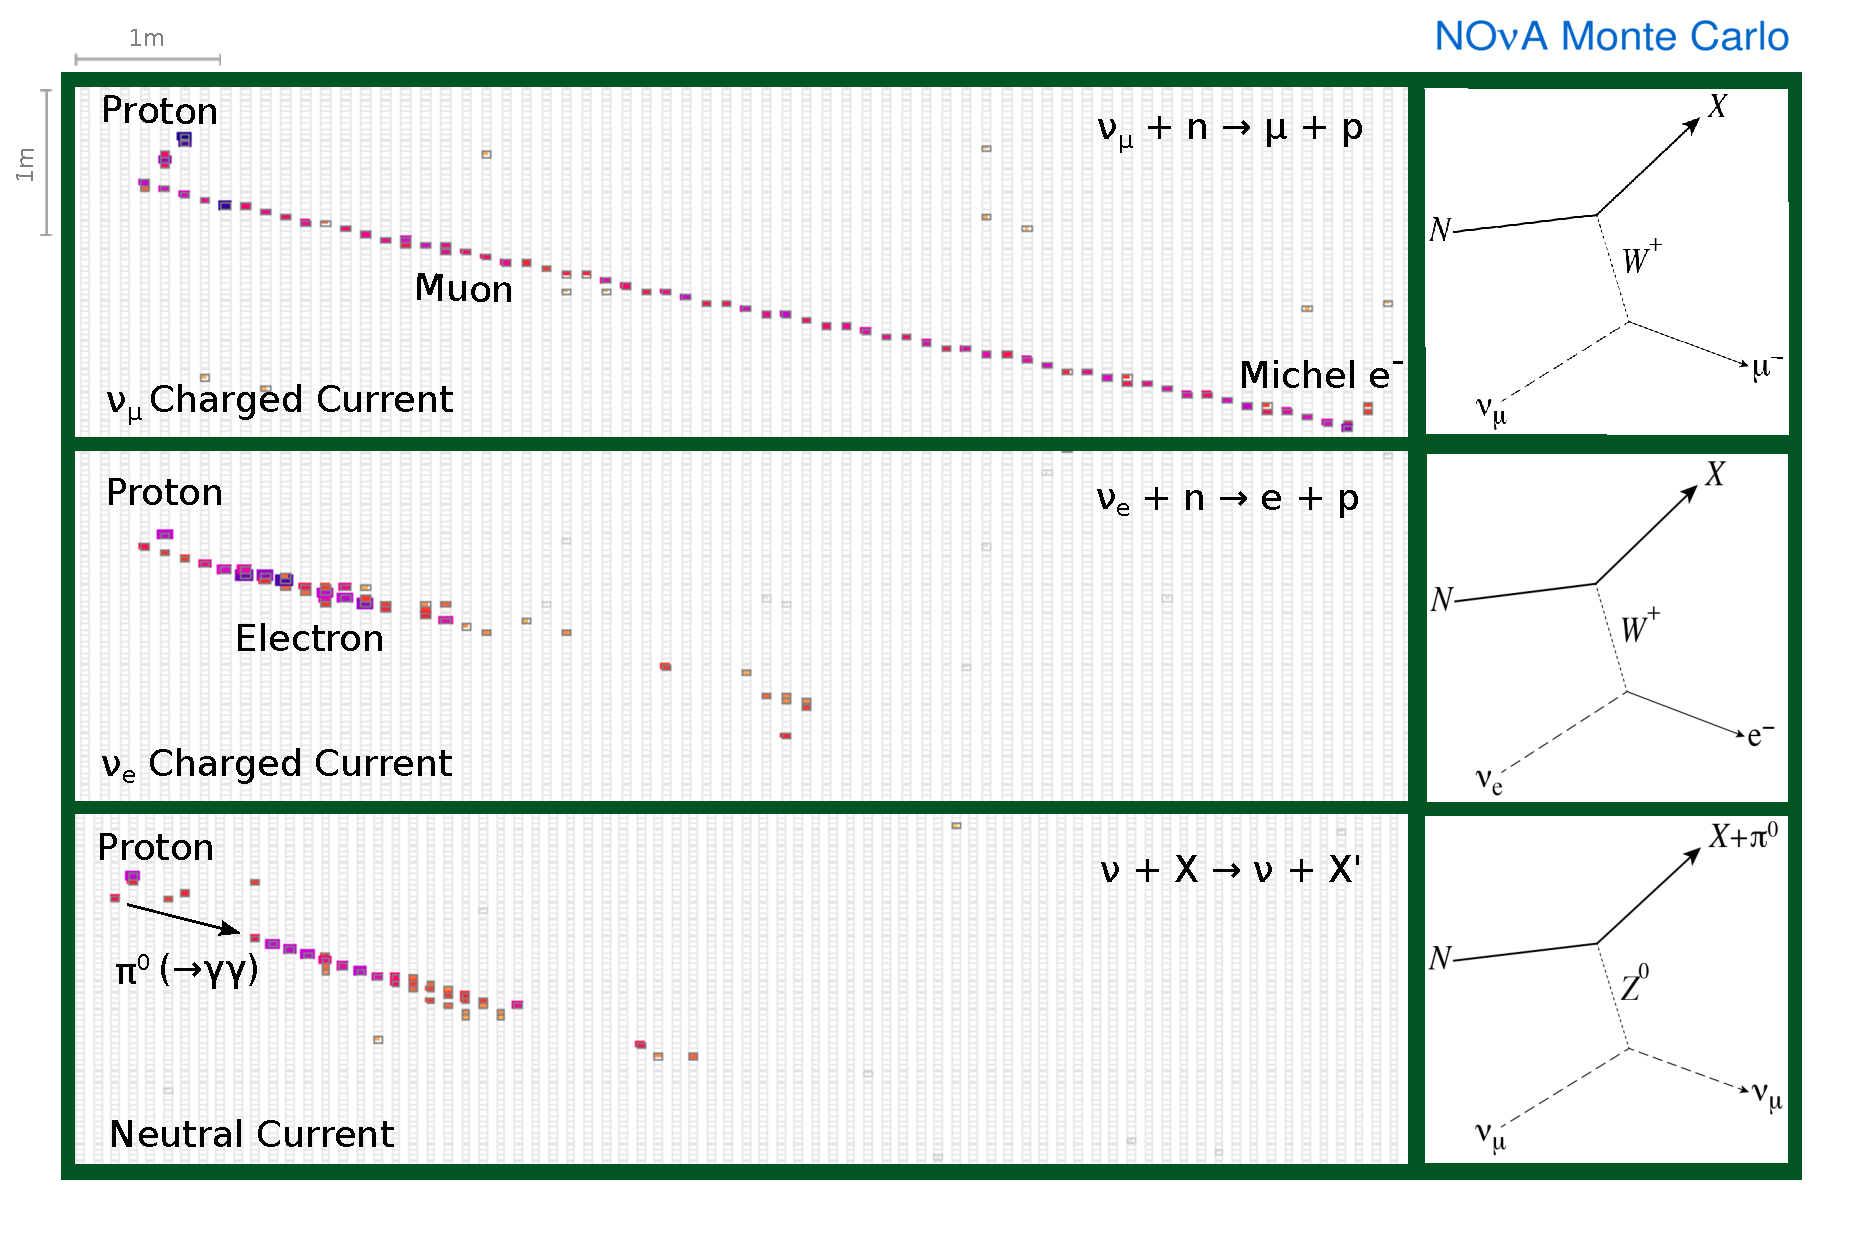
\includegraphics[width=1\textwidth]{/home/robert/Documents/School/PhD/Thesis/Plots/NOvAExperiment/NOvAEventTopology.pdf}
\caption[NOvA detectors event topologies]{Different event topologies as seen in the \acrshort{NOvA} detectors with corresponding Feynman diagrams \cite{NOvAReco.pdf}. Each event is a simulated $\unit[2.15]{GeV}$ neutrino interacting in a \acrshort{NOvA} detector producing a $\unit[0.78]{GeV}$ proton and a second $\unit[1.86]{GeV}$ particle depending on the interactions type. The figure show one view and the colouring represents the deposited energy.}
\label{fig:NOvAEventTopologies}
\end{figure}

NOvA employs a \gls{CNN} based on the GoogLeNet \cite{GoogLeNetArchitecture.pdf} architecture named \gls{CVN} \cite{CVN.pdf}, which uses slice hits to classify interactions into one of the four categories: $\nu_e$, $\nu_\mu$, $\nu_\tau$, or \gls{NC}. The same architecture, but applied to the Fuzzy-K prongs and called \textit{ProngCVN} \cite{PhihasNOvAThesis_ProngCVN.pdf}, is used to identify the individual prongs based on what particles they most likely correspond to. A special \gls{ML} algorithm for identifying muons, based on a \gls{BDT} with inputs from the Kalman track, is called \gls{ReMId}~\cite{RaddatzNOvAThesis_KalmanTracks.pdf}.

%From First NOvA results on FHC+RHC: These clusters are categorized as electromagnetic or hadronic in origin using a convolutional neural network (CNN) [Fernanda Psihas thesis]. Hits forming tracks are identified as muons by combining information on the track length, dE=dx, vertex activity, and scattering into a single particle identification (PID) score [Raddatz thesis].

%From NOvAHalfTimeOverview2022.pdf: The energy of charged current neutrino interactions is estimated from the sum of energies of the lepton and the hadronic recoil system. A Kalman-like algorithm is used with a BDT based on energy loss, multiple scattering, and length parameters of a candidate track to identify muons and reconstruct their energy using track length. The energy of electron neutrinos is estimated from a quadratic function of the calorimetric energies of the electron candidate and the hadronic recoil system derived from the simulation [33, 34].

%%%%%%%%%%%%%%%%%%%%%%%%%%%%%%%%%%%%%%%%%%%%%%%%%%%%%%%%%%%%%%%%%%%%%%%%%%%%%%%
%%%%%%%%%                   Detector calibration                     %%%%%%%%%%
%%%%%%%%%%%%%%%%%%%%%%%%%%%%%%%%%%%%%%%%%%%%%%%%%%%%%%%%%%%%%%%%%%%%%%%%%%%%%%%
\section{Detector Calibration}\label{sec:NOvACalibration}
%%% General introduction to calibration - why do we do calibration? What do we get from the DAQ?
The energy deposited within the NOvA detectors is represented by the peak \gls{ADC} values for each cell the particle passed through, which are obtained from the readout electronics, as described in Sec.~\ref{sec:DAQ}.
To convert \gls{ADC} into physical units we need to calibrate the \gls{NOvA} detectors \cite{PrabhjotNOvAThesis_CalibrationAndOscResults2019.pdf}, while accounting for the attenuation of light along the \gls{WLS} fibres, or for differences between individual cell. The purpose of calibration is to calculate a conversion factor from $\unit{ADC}\rightarrow\unit{MeV}$ units, so that the same energy deposited at any place within any detector and at any time, is recorded as the same value.
%By doing this individually for each cell and for small periods at a time, we ensure that energy deposited in any detector, at any place within the detector and at any time, is recorded as the same value in physical units.

%From NOvAHalfTimeOverview2022.pdf: The variations in light output between cells and those due to attenuation along the readout fiber, in both data and simulation, are calibrated using cosmic-ray muons. The overall energy response of the detectors is calibrated using stopping muon tracks along a window from 200 cm to 100 cm before the end of the track. The absolute energy scale is cross-checked and bench marked against simulation using beam-induced protons, muons, and neutral pions at the Near Detector.

%make sure that we get the same amount of energy wherever or whenever it's deposited in whichever of NOvA's detectors and to express this amount of energy in physical units. The NOvA calibration uses cosmic ray muons, which provide a consistent, abundant, and well-understood source of energy deposition.

%%% Calibration samples, trigger, reconstruction, and selection. Also simulation, fiber brightness and so on...
\gls{NOvA} uses cosmic ray muons for calibration due to their abundance in the \gls{NOvA} detectors and a consistent energy deposition. We use hits from muons stopping inside the detectors, from a window when they are almost exactly \gls{MIP}, to calculate the absolute energy scale. The cosmic muons are collected using a periodic data-driven trigger, removing events with timestamps overlapping with the beam spill window. For the simulation of cosmic muons we use the CRY~\cite{CRY} \gls{MC} generator, as outlined in Sec.~\ref{sec:NOvASimulation}.

\note{I talk about this selection later on in the Test Beam calibration chapter when I talk about the data-based simulation. Should I therefore elaborate more on this or is this enough?}
We reconstruct the cosmic muon tracks using the window cosmic track algorithm explained in Sec.~\ref{sec:NOvAReconstruction}. To select good quality cosmic tracks we require that at least $80\%$ of all hits from the reconstructed slice contribute to the track \cite{NOvA-doc-13579-FACalorimetricEnergyScale}. Additionally, all tracks must cross at least $\unit[70]{cm}$ along the z axis and must have at least $20\%$ of their total track direction in the z axis, since very vertical tracks tend to not be reconstructed well. \note{There are additional selection criteria which are not as important, do I need to mention them?}. To select stopping muons we look for Michel electrons, which get produced by decaying muons at the end of their tracks, as can be seen on the top panel of Fig.~\ref{fig:NOvAEventTopologies}.

The energy deposited in a cell is proportional to the distance the particle travels through the cell. To ensure we use precise estimate of the path length, we only use hits that satisfy the \textit{tri-cell} condition, shown on the left of Fig.~\ref{fig:NOvATricellCondition}. This means that each hit must have a corresponding hit in both of the surrounding cells in the same plane. This allows us to calculate the path length simply from the height of the cell and the angle of the reconstructed track. In case there is a bad channel in a neighbouring cell (right side of Fig.~\ref{fig:NOvATricellCondition}), we ignore this channel and look one cell further. We can then calculate the path length simply as the cell width divided by the cosine of the direction angle \cite{PrabhjotNOvAThesis_CalibrationAndOscResults2019.pdf}.

\begin{figure}[hbtp]
\centering
\begin{subfigure}[b]{0.49\textwidth}
\centering
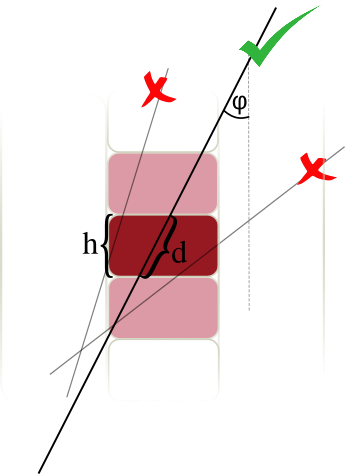
\includegraphics[width=0.6\textwidth]{Plots/NOvAExperiment/TricellConditionWithDescription.png}
\end{subfigure}
\begin{subfigure}[b]{0.49\textwidth}
\centering
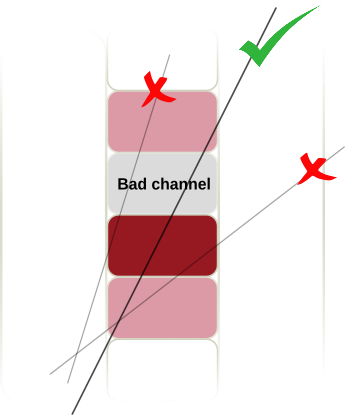
\includegraphics[width=0.6\textwidth]{Plots/NOvAExperiment/TricellConditionWithBadChannel.png}
\end{subfigure}
\caption[Tricell condition for calibration hits in NOvA]{Illustration of the tricell condition. We only use hits that have two surrounding hits in the same plane to be used in the \acrshort{NOvA} calibration, shown on the left plot. This is to ensure a good quality of the path length (d) reconstruction, which is calculated from the known cell height (h) and the reconstructed track angle $\left(\varphi\right)$. In case the hit is next to a bad channel, as shown on the right plot, we ignore this bad channel and require a hit in the next cell over.}
\label{fig:NOvATricellCondition}
\end{figure}

%The first step in the attenuation calibration is to select the suitable hits from tracks of cosmic ray muons. Because a reliable estimate of pathlength is required, not all hits are suitable for use.  If a cell has each of its neighbors in the same plane hit, then we know, for a Y view cell, that the track entered through the upper wall, and exited through the lower wall. The pathlength then is just the width of the cell divided by the direction cosine. This selection also significantly decreases the chance that the hit in question is a noise hit. Allowance is made for neighboring dead cells, so e.g. “hit, dead, hit, hit” would still lead the 3rd cell to be selected. The second best hit selection, in cases where there are too many dead neighboring cells on each side, is the so-called “z” estimator, where a hit is required at the same cell number in each of the neighboring planes in the same view. The pathlength is then the ratio of cell depth to cz.[docdb:13579 - SA The Attenuation and Threshold Calibration of the NOvA detector, copied from docdb:7410]

%from docdb:7410: A requirement that the track be “throughgoing” (lowest endpoint outside the fiducial volume) was applied, but doesn’t make much difference. I think this selection was broken by the recent changes to StopperSelection anyway. (So it seems that it was required for the relative calibration that the muons are through-going, but I assume this was discarded somewhere down the line)

%Stopping muon selection (from docdb:13579 - FA\_Calorimetric\_energy\_scale): There are two avenues for selecting stopping muons; i) selecting tracks whose reconstructed end point is contained within the detector and ii) selecting tracks that have a Michel electron at one end. Michel electrons are useful for both identifying muons and effective tagging of the end point of muon tracks. The stopping selection requires the reconstructed end point of the muon track to be at least 50 cm from the detector edge. The identification of a Michel electron at the end of a muon track has two stages of both temporal and spatial range requirements. Firstly, a candidate Michel electron hit is required to occur between 1 and 30 microseconds after the mean time of the hits on the track. Furthermore, the candidate Michel electron must be within a 30 cm sphere surrounding the reconstructed track end point. The candidate Michel electron hit for a muon track is the hit that produces the largest detector response among the hits that pass the above cuts. Secondly, cell hits surrounding the candidate Michel electron hit are associated with the Michel electron if they occur within a 30 cm sphere surrounding the Michel electron candidate. Furthermore, to be associated with the Michel electron the cell hits must occur between 0.5 microseconds before and 0.5 microseconds after the candidate Michel electron. Michel electrons at the end of muon tracks are reconstructed using the candidate and associated Michel electron hits. The stopping muon selection requires a Michel electron at the end of the muon track.

%Calibration is necessary to convert electronic signals to physically meaningful energy in units of GeV. Two calibration steps precede the calorimetric energy calibration. First raw ADCs (Analogue Digital Conversion) are converted to units of photo-electrons (PE) using the known average response of the APDs; secondly an attenuation calibration corrects for the position dependent response [6]. A drift calibration may be included in the future to correct for changes in detector response over time. The calorimetric energy scale calibration is the last step in the calibration chain and the detector response should already be uniform in space and eventually also in time. [docdb:13579 - FA\_Calorimetric\_energy\_scale]

%Using the average expected APD response, integrated charge from the ADCs are converted to units of photo-electrons (PE) [SA Absolute energy scale]

The calibration conversion factor from the signal recorded by the detector readout and the actual deposited energy can be expressed by Eq.~\ref{eq:NOvACalibration}.
\begin{equation}\label{eq:NOvACalibration}
E_{dep}\ \left[\unit{MeV}\right]=\textsf{Signal}\ \left[\unit{ADC}\right]\times S_d\times TS_{d,i}\times R_{d,i}\left(t\right)\times A_d\left(t\right).
\end{equation}
Here we can see that calibration consists of four separate and complementary factors: the Scale $\left(S_d\right)$, the Threshold/Shielding correction $\left(TS_{d,i}\right)$, the Relative calibration $\left(R_{d,i}\left(t\right)\right)$ and the Absolute calibration $\left(A_d\left(t\right)\right)$, all described below. Each part is calculated for each detector separately, as indicated by the subscript $d$. The Relative and Absolute calibrations are calculated for each time period separately to account for possible changes in the energy deposition throughout the time, possibly caused by the ageing of the scintillator oil, or of the readout electronics. The time periods are either determined by running conditions and separated by significant changed to the readout or \gls{DAQ} systems, including the summer shutdown, or by a fixed time interval.

The Threshold/Shielding correction and the Relative calibration calculate a calibration factor for each position within the detector to account for variations caused by the attenuation of light as it travels through the \gls{WLS} fibres, or by differences between individual cells. This is denoted as a subscript $i$ in Eq.~\ref{eq:NOvACalibration}. For data, the position of hit in a detector is described by the plane number, the cell number and the position within the cell $\left(w\right)$. $w$ is calculated as the projection of the cosmic track to the central cell axis and its value is equivalent to the X axis (Y axis) coordinate of the projection for the horizontal (vertical) cells, with the 0 value at the centre of the cell \cite{PrabhjotNOvAThesis_CalibrationAndOscResults2019.pdf}.

%The light is attenuated while traveling through the fiber. To find the correct energy of the incident particle these losses are corrected by using cosmic ray muons. The cosmic ray muons are used to calibrate the NOvA detectors because they provide a source of consistent energy across the detectors. The purpose of the attenuation calibration is to provide constants and formulae such that an amount of energy deposited in the detector and registered by an APD can be expressed in comparable units, PECorr which are the corrected photo-electrons (PE) no matter where the deposition occurred. Variations in time are to be handled by the drift calibration. The purpose of the absolute calibration is to provide a scaling factor, independent of channel since all of that variation should have been taken out by the relative calibration, so that energy deposits can be expressed in physically meaningful units (GeV).
%For both purposes cosmic rays are used as probes. For the attenuation calibration they represent a source of consistent energy deposits across the detector of approximately 1 minimum ionizing particle’s energy, MIP, but this is not assumed. Any average value consistent across the detector would do. For absolute calibration, stopping muons are used, whose precise energy deposits should be estimateable from the Bethe Bloch formula. [docdb:13579 - SA The Attenuation and Threshold Calibration of the NOvA detector, but a lot of this is actually just copied from Backhouse's original calibration technote docdb:7410]

%(Dividing data into periods and epochs) A new period is started for a major change to running conditions such as a horn current change, a long shutdown, target replacement, etc. Periods are divided into epochs. A new epoch is started whenever analysis or production reasons dictate. Calibration has been performed for all the periods separately and has used the data that are determined by the Data Quality group to be good. The effects of aging, temperature, partial filling, and cooling are neglected. The drift calibration should be able to account for all of these (but drift calibration doesn't really exist yet afaik). [docdb:13579 - SA The Attenuation and Threshold Calibration of the NOvA detector]

For simulation, we do not use the plane number to determine the position within a detector, as by construction all detector planes should have the exact same readout. This significantly reduced the requirements for the number of events that need to be simulated, reconstructed and calibrated, especially for the \gls{FD} with 896 planes. However, in reality there are some variations in detector response between individual planes, caused by different \textit{brightness} qualities of the fibres, zipped or twisted fibres, different qualities of the scintillator, possible air bubble, or potentially others. Since we want to include these differences into simulation without having to simulate every cell individually, we divide all cells into 12 equally populated \gls{FB} bins based on
the uncorrected average response in the center of that cell, as shown on Fig.~\ref{fig:NOvAFiberBrightness}. These brightness bins describe the relative differences in the detector response between individual cells \cite{NOvA-doc-34909}.

%\cite{NOVA-doc-13579-SAAttenuationAndThreshold,NOVA-doc-34909}.

\begin{figure}[hbtp]
\centering
\begin{subfigure}[b]{0.495\textwidth}
\centering
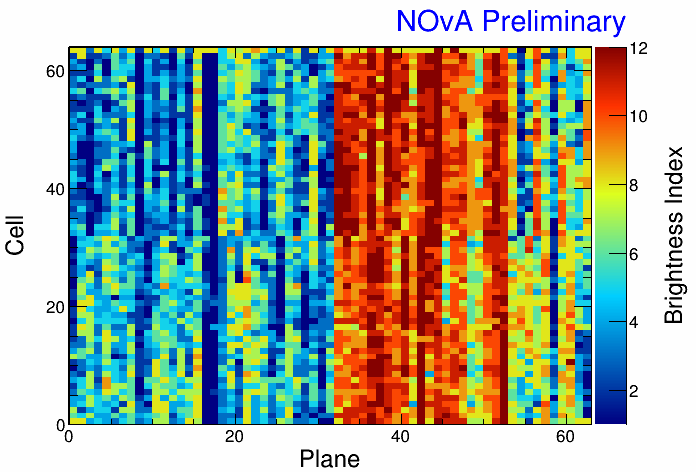
\includegraphics[width=\textwidth]{Plots/NOvAExperiment/BrightnessIndex.png}
\end{subfigure}
%\hfill
\begin{subfigure}[b]{0.495\textwidth}
\centering
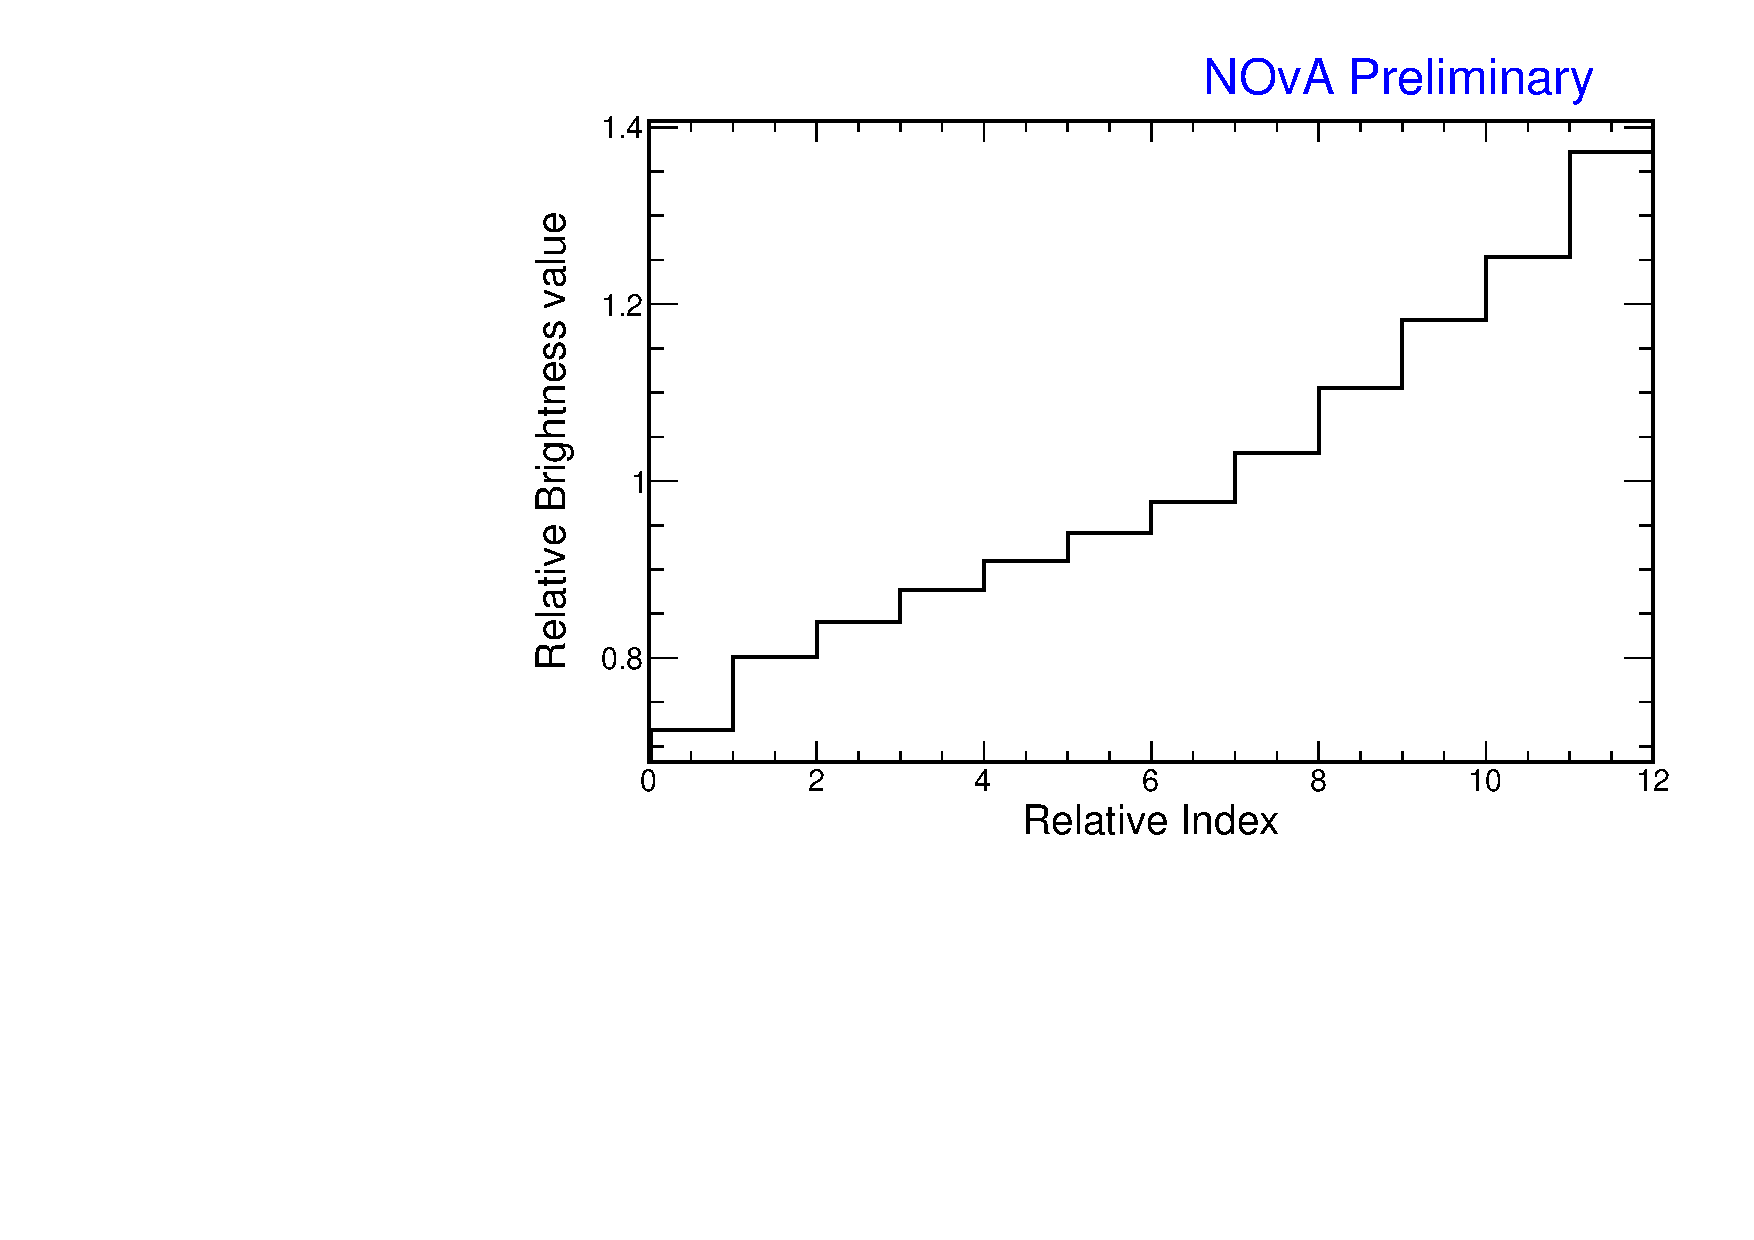
\includegraphics[width=\textwidth]{Plots/NOvAExperiment/BrightnessIndexToValue.pdf}
\end{subfigure}
\caption[Fibre Brightness bins for the NOvA calibration]{Distribution of the \acrshort{NOvA} detector cells into 12 brightness bins (left plot), each representing a relative difference in energy response (right plot) due to different brightnesses of the fibres, scintillators, or readout. This is an example from the \acrshort{NOvA} Test Beam detector, where the left side of the detector (planes 1-32) has clearly lower response relative to the right side of the detector (planes 33-64).}
\label{fig:NOvAFiberBrightness}
\end{figure}

%To divide each detector into the 12 brightness bins, we use results from the relative calibration. Specifically we take the result of the attenuation fit (equal to the average response) in the centre of each cell to fill a 2D histogram. Then we normalize this histogram by dividing the response in each $\textsf{Cell}\times\textsf{View}\times\textsf{Plane}$ by the average response in the corresponding $\textsf{Cell}\times\textsf{View}$. All uncalibrated cells get assigned the average response (1 in normalized histogram). Then we make a 1D histogram filled with the normalized responses of each cell and divide this histogram into 12 equally populated bins (so each bin represents approximately the same number of detector cells, shown on the left plot of Fig. \ref{figFiberBrightnessBins}). The mean normalized response in each bin represents the relative brightness value of this bin (right plot of Fig. \ref{figFiberBrightnessBins}).

\subsection{Scale}
The Scale calibration factor from Eq.~\ref{eq:NOvACalibration} is a simple conversion from the peak \gls{ADC} value into the number of \gls{PE}s. This factor only depends on the \gls{APD} gain (which was different in the beginning of \gls{NOvA} data taking) and on the FEB type (different between detectors, as described in Sec.~\ref{sec:DAQ}).

%I think I should actually include some kind of a description of the ADC to PE conversion.
\iffalse
The scaling of the ADC to PE depends only on the gain and the version of the FEB. Otherwise it's just a very simple scaling (explain this at the PE definition):
\begin{equation}
PE=\frac{\textsf{peakADC}}{\textsf{ADCPerPE}},
\end{equation}
\begin{equation}
\textsf{ADCPerPE}=\textsf{Gain}\times\frac{4095}{ADCScale}
\end{equation}
where ADCScale is 217000 for FEBv4.1 and 204800 for FEBv5.2.
\fi

%The PECorr scaling is 75.0 (NDOS), 37.51 (ND), 39.91 (FD) and 39.91 (TB)

\subsection{Threshold and shielding correction}
%[CalibrationFirstTechnote2014.pdf] There are three main assumptions for calibration: response is stable in time (drift), the energy spectrum of cosmic rays is uniform in space (shielding), the ADC response to arriving photons is linear

The Threshold and Shielding correction accounts for two assumptions, which hold true in most cases in NOvA, but fall short for some hits at the bottom of the detector, or far away from the readout, especially for the \gls{FD} \cite{PrabhjotNOvAThesis_CalibrationAndOscResults2019.pdf}. The first assumption is that the \gls{ADC} response to the photon signal is linear, which is mostly true except close to the \gls{APD} threshold. Energy deposited far away from the readout may produce photons that get attenuated enough to be shifted below the threshold. However, due to natural fluctuation, the same deposited energy may also produce photons that would make it over the threshold, therefore making it appear that the actual deposited energy was higher then in reality, introducing a bias to the calibration. The threshold correction is calculated using simulation, as the ratio between the number of simulated \gls{PE} seen by the \gls{APD} $\left(\textsc{PE}_{true}\right)$ and the Poisson mean number of simulation photons created in the scintillator by the same deposited energy $\left(\lambda\right)$.

The second assumption is that the spectrum of cosmic muons is uniform within each detector. Again, this is generally true, but breaks down at the \gls{FD}, which is big enough that the top of the detector shields the bottom part of the detector and affects the energy distribution. The shielding correction is calculated from simulation as a ratio between the true energy deposited by a charged particle $\left(E_{true}\right)$ and the expected deposited energy if the particle was \gls{MIP} $\left(E_{\textsc{MIP}}\right)$. 

The total Threshold and Shielding correction is calculated for simulated events in each cell, \gls{FB} bin and $w$ position according to Eq.~\ref{eq:NOvAThresholdShieldingCorrection}. The final correction is a fit to the mean correction value along $w$ in each cell and \gls{FB} bin.

\begin{equation}\label{eq:NOvAThresholdShieldingCorrection}
TS_i = \frac{\textsc{PE}}{\lambda}\frac{E_{true}}{E_{\textsc{MIP}}}.
\end{equation}

%Similar effect, specifically for the vertical cells, is caused by using cosmic muons for calibration and applying it to beam muons. The top of the detector effectively shields the bottom, skewing the energy distribution of cosmic muons. To correct for both of these effect, we use the simulation pclist sample to calculate the threshold and shielding (also called threshold and shadowing) correction by comparing the true and reconstructed information. We apply this correction before the attenuation fits \cite{NOVA-doc-13579-SAAttenuationAndThreshold}.

%Should I write anything more? Maybe about how do we calculate this more specifically, or that it's done for view X fb bin X cell X w

%In the Far Detector data and MC a large divergence between calibrated and true energies as a function of W was observed [8]. This was traced back to the much longer cell lengths in the FD meaning that thresholds play a large role at the foot of a cell. Also self-shielding of the detector by its own mass lay a role in the observed discrepancy. Thresholds mean that for a hit to be seen by an APD, it may need to have a slight upwards fluctuation in the number of photons produced by the energy deposition. Self-shielding means that the average visible energy depositions from MIPs are not truly spatially uniform in the detector. If not corrected for these effects, there will be a bias in the set of hits that the attenuation fit sees, and leads it to overestimate the light-level, and so under-estimate real hit energies by tens of percent. The approach adopted to solve this problem was to create a correction factor as a function of view, cell, and position along the cell which would be applied before the attenuation correction to remove the effect of thresholds and shielding. To this end MC truth information about the calibration hit sample is used to create a combined threshold and shadowing correction for each cell and view combination,
%\begin{equation}
%T=\frac{PE}{\lambda}\frac{E_{true}}{E_{mip}},
%\end{equation}
%where $T$ is the combined “threshold and shielding” correction factor, $PE$ is the simulated photoelectrons recorded at the readout, $\lambda$ is the number of simulated photons which would be seen at the readout out in the absence of fluctuations, $E_{true}$ is the true energy deposited in the cell and $E_{mip}$ is the naive energy you would expect to be deposited based on the pathlength through the cell. In this way it encodes a threshold correction based on the simulated readout PE with and without the fluctuations, with $\lambda$ dependent on your simulated threshold, as well as a shielding correction based on the simulated energy deposition and a naive no shielding approximation. This equation gives us a cell by cell correction but we use an empirical polynomial fit to that distribution which removes statistical noise from the correction and well describes the initial distribution. This correction factor is applied to the cell by cell data and MC PE/cm distributions before the attenuation fits. [docdb:13579 - SA The Attenuation and Threshold Calibration of the NOvA detector, reference 8 is for docdb:7247, a talk by Backhouse]

\subsection{Relative calibration}\label{secRelativCalibration}

%The \textbf{relative calibration} corrects for attenuation of scintillator light as it travels through the cell to the readout, as well as for differences between detector cells. This correction is calculated for each cell separately.

%Detailed description can be found in the "Instructions for the Attenuation Calibration Job" technote from Prabhjot from docdb:13579 (list of all calibration technotes) and on the relative calibration wiki page.

Relative calibration corrects mainly for the attenuation of the scintillator light as it travels through the \gls{WLS} fibre to the readout. Since to correction is calculated for each cell independently, it effectively correct for the relative differences between detector cells as well. The result of the Relative calibration is the detector response to a particle in the units of \gls{PECorr}, which is calculated as the ratio between an average response in \gls{PE} across the entire detector (can differ across detectors) and the result of the \textit{"attenuation fit"} in that particular position within the detector. This way the \gls{PECorr} should be uniform across the detector along the plane number, cell number and $w$ distributions \cite{PrabhjotNOvAThesis_CalibrationAndOscResults2019.pdf}.

%by fitting the average detector response over the position in each cell, separately for every cell inside each detector. Dividing the "average response" of the detector by the result of the attenuation fit for each $\textsf{Plane}\times\textsf{Cell}\times\textsf{w}$ combination effectively removes relative differences within and between all cells across the entire detector. The average response is a single constant number chosen to approximately represent the average response in the middle of the cell. Its value is for the far detector and Test Beam 39.91~PE/cm and for the near detector 37.51~PE/cm. The value of the average response has no impact of the calibration results, as the absolute scale of the detector response is determined during the absolute calibration and relative calibration only serves to remove the relative differences \cite{NOVA-doc-7410,NOVA-doc-13579-SAAttenuationAndThreshold}.

To do the attenuation fit, we first create the \textit{"attenuation profiles"} for each detector cell. Attenuation profiles are profile histograms of mean detector response over the travelled path length, in the units of $\textsc{PE}/\unit{cm}$, along the position within the cell. An example attenuation profile is shown on Fig.~\ref{fig:NOvACalibrationAttenuationFit} as black dots. We then apply the Threshold and Shielding correction described above before doing the attenuation fit, which consists of two steps. 

\begin{figure}
    \centering
    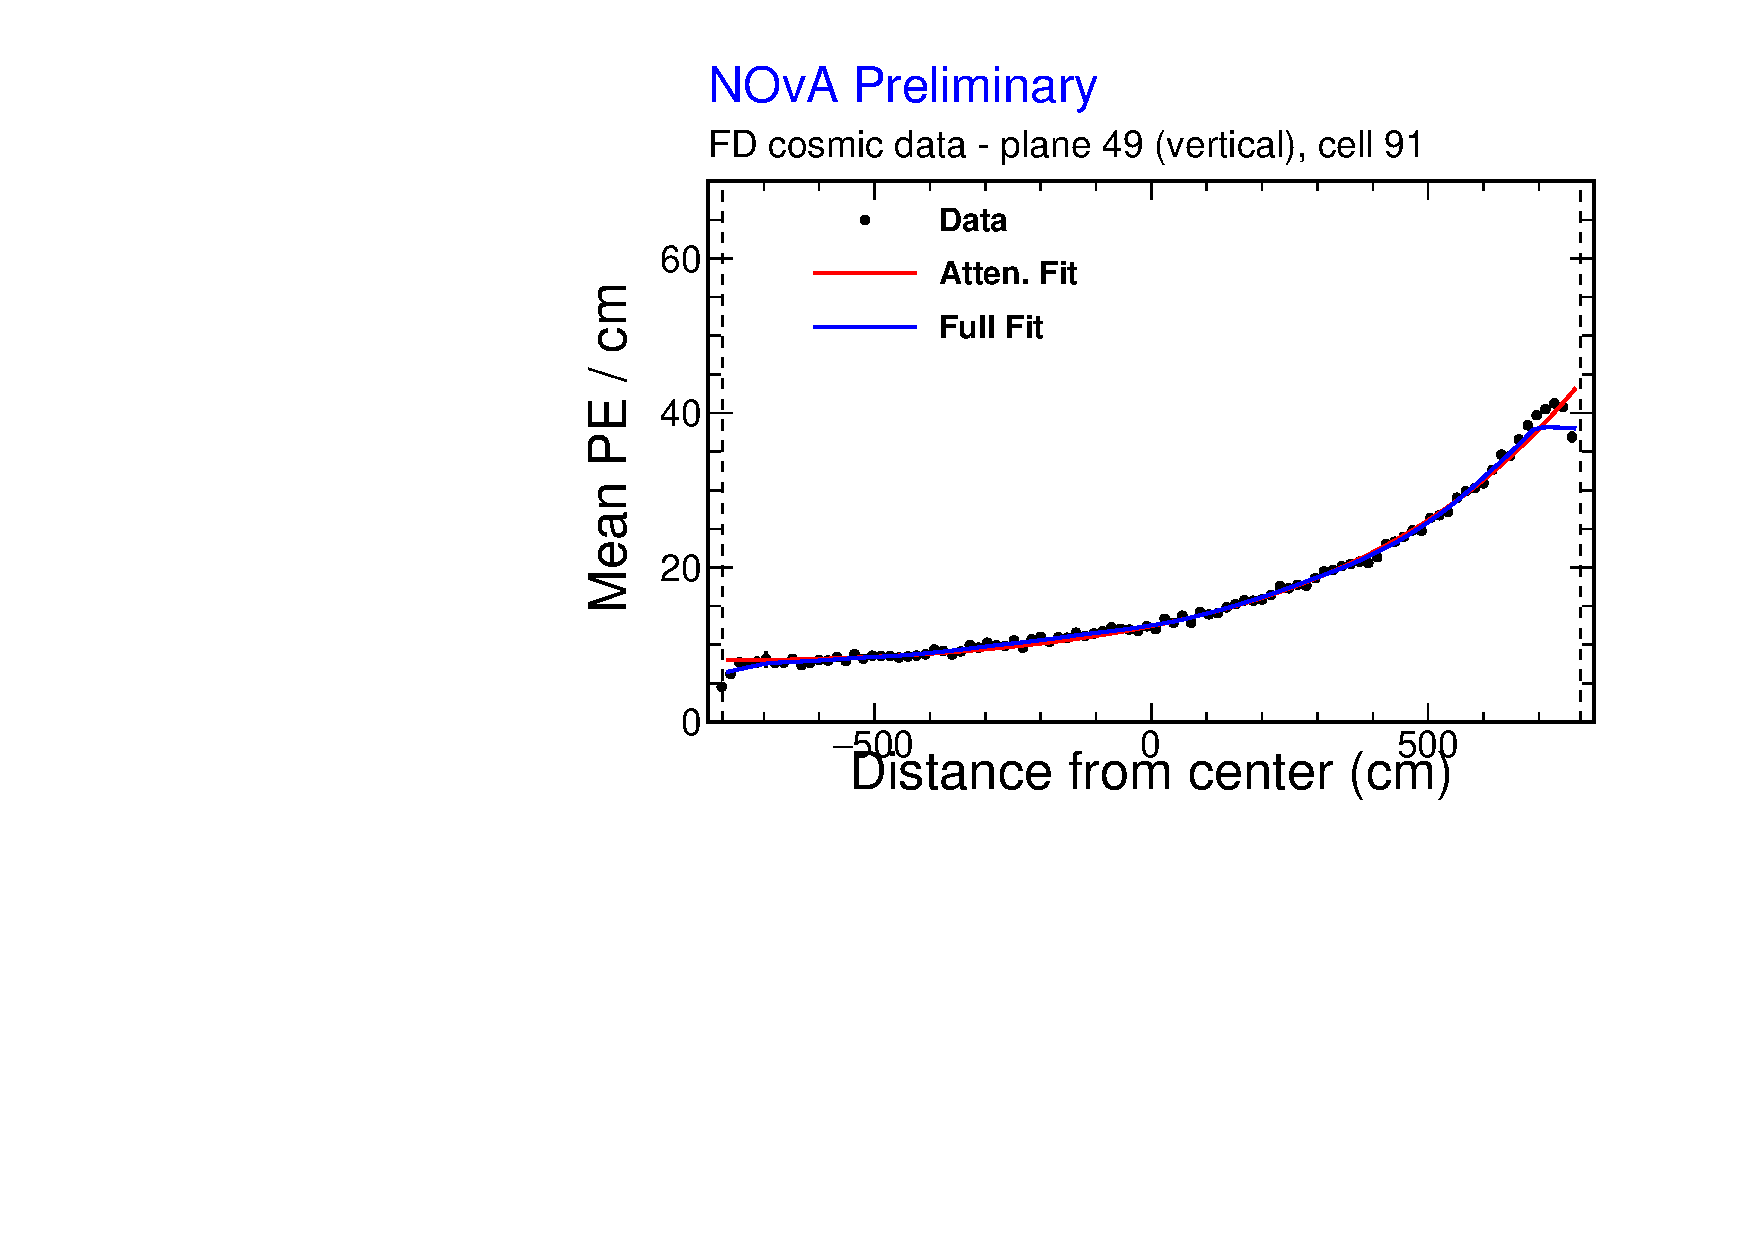
\includegraphics[width=.7\textwidth]{Plots/NOvAExperiment/ExampleAttenuationFit.pdf}
    \caption[Example attenuation fit for NOvA Relative calibration]{Example attenuation fit for a single cell in the \acrshort{NOvA} \acrshort{FD} across its full length, as shown by dashed vertical lines. The red line shows the initial exponential fit and the blue line shows the full fit after the \acrshort{LOWESS} correction, both described in text. Figure from \cite{totfit_fd_datafitX_049_091.pdf}.}
    \label{fig:NOvACalibrationAttenuationFit}
\end{figure}

\begin{enumerate}
\item The first step is a three-parameter exponential fit according to Eq.~\ref{eq:NOvARelCalibExpFit}
\begin{equation}\label{eq:NOvARelCalibExpFit}
y=C+A\left(\exp\left(\frac{w}{X}\right)+\exp\left(-\frac{L+w}{X}\right)\right),
\end{equation}
where $y$ is the fitted response, $L$ is the length of the cell and $C$, $A$ and $X$ are the fitted parameters representing the background, attenuation scale and attenuation length respectively. An example of the exponential fit is shown as a red curve on Fig.~\ref{fig:NOvACalibrationAttenuationFit}.
\item The second step is smoothing out of the residual differences between the exponential fit and the original distribution with the \gls{LOWESS} method, shown on Fig.~\ref{fig:NOvACalibrationLOWESSCorrection}. We use 20 points across the length of each cell to create a smoothed distribution of the residual values. Result of the \gls{LOWESS} correction is then combined with the exponential fit into the full attenuation fit, shown as a blue line on Fig.~\ref{fig:NOvACalibrationAttenuationFit}.
\end{enumerate}

\begin{figure}
    \centering
    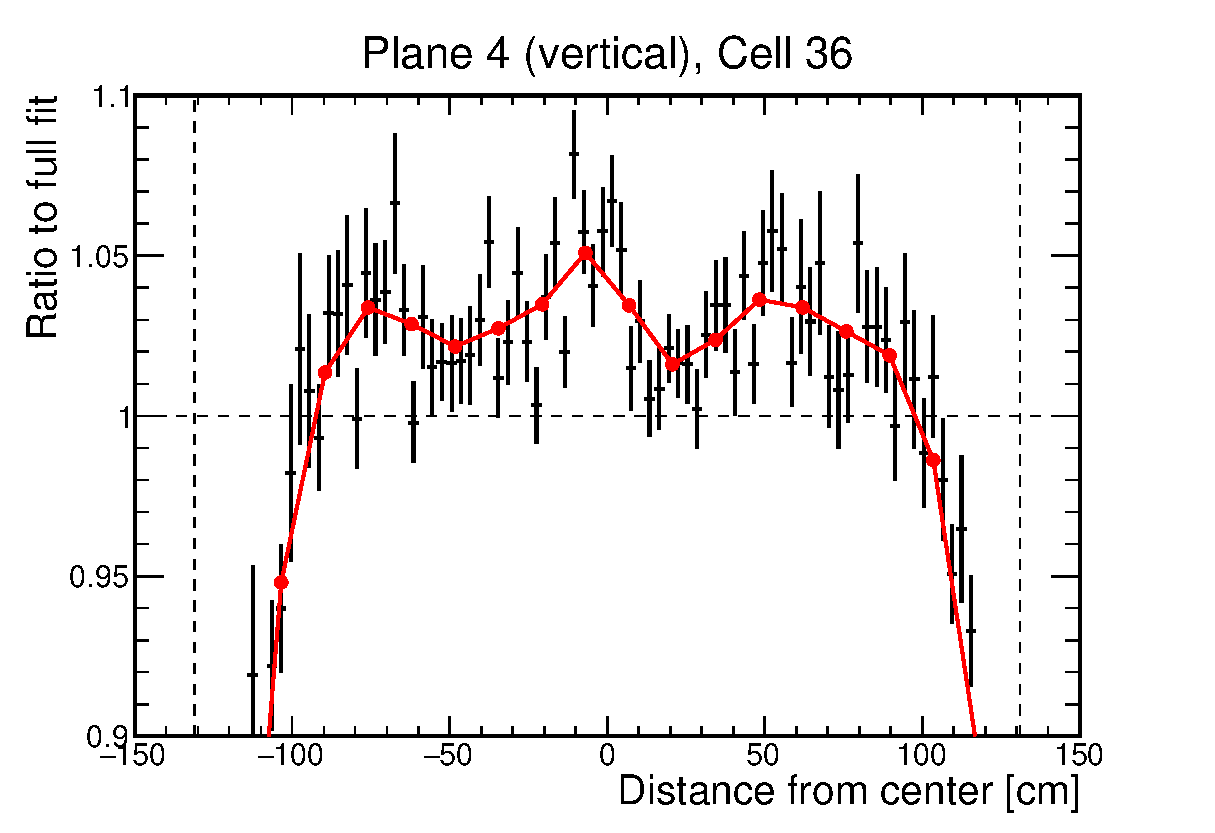
\includegraphics[width=.7\textwidth]{Plots/NOvAExperiment/ExampleLOWESSFit.eps}
    \caption[Example LOWESS correction for NOvA Relative calibration]{Example \acrshort{LOWESS} correction for a the residual differences after the exponential part of the attenuation fit of the \acrshort{NOvA} Relative calibration. This is an example for a single cell in the \acrshort{NOvA} \acrshort{TB} detector with black point showing the residual differences and red line the \acrshort{LOWESS} correction, both described in text.}
    \label{fig:NOvACalibrationLOWESSCorrection}
\end{figure}

Even after an application of the \gls{LOWESS} correction, there are sometimes large differences between the attenuation fit and the fitted response. This is usually caused by a small number of events in that cell, common for cell at the edge of the detector. To ensure a good quality of the attenuation fit, we calculate the total $\chi^2$ between the attenuation fit and the fitted response and only call a cell \textit{calibrated}, if the final $\chi^2<0.2$. If $\chi^2>0.2$, we ignore the results for this cell and mark it as \textit{uncalibrated}.

%Attenutation profiles have a constant binnin fNBins=100 (in w), same for ND, FD and TB. This results in an effectively finer binning for TB compared to ND and FD. For FD w = (-900,+900), ND: (-250,+250), TB: (-150,+150). TB: 3cm/bin, ND: 5cm/bin, FD: 18cm/bin. What effect could this have on the relative calibration results? Particularly on the calibration shape?

%where y is the response, L is the cell length, C, A and X are the free parameters in the fit. X gives the attenuation length as well. Initially, the fit is to the central part of the cell, which is different for each detector. In addition to the approximately quartic behavior at the ends of every channel there are in many channels fairly large residuals. They don’t appear to follow any consistent pattern. The leading hypothesis is that these are due to varying fiber position within the cell. Usually the fiber lies in the corners of the cell, but if it is somehow twisted so that it rises into the center of the cell, then it should collect more light, to an extent comparable to what is seen here. To remove such an irregular pattern, the residual from the analytic fit is simply fit with LOcally WEighted Scatter plot Smoothing, LOWESS. The LOWESS curve at each point is formed from the weighted mean of the deviations. The weighting function is the traditional tri-cube, (insert equation, likely not needed for this technote) [docdb:13579 - SA The Attenuation and Threshold Calibration of the NOvA detector, already in 1stAna and Backhouse's technote]

%For NDOS the fit was a very little bit different, where we didn't use $L$ but $3L/2$. Also it says that "Over the length of an NDOS cell, the effect of the long attenuation length is imperceptible, and is modelled as a constant (If you put a long attenuation term in, the fit drives the length scale to infinity anyway). [docdb:7410]

%In many channels, fairly large residuals are visible. They don’t appear to follow any consistent pattern. The hypothesis is that these are due to varying fibre position within the cell. Usually the fibre lies in the corners of the cell, but if it is somehow twisted so that it rises into the centre of the cell, then it should collect more light, to an extent comparable to what is seen here. To remove such an irregular pattern, the residual from the analytic fit is simply fit with LOWESS (locally weighted scatterplot smoothing). The LOWESS curve at each point is formed from the weighted mean of the deviations. The weighting function is the traditional tri-cube:
%\begin{equation}
%w_i=\left(1-\left|\frac{x-x_i}{\sigma}\right|^3\right)^3.
%\end{equation}
%The smoothing length scale $\sigma$ is 30cm. 20 points calculated by this method are stored, to be linearly interpolated between to approximate the full LOWESS curve. If the LOWESS fit at any point exceeds 15\% the original attenuation fit was very bad, and the channel is marked uncalibrated. Figure 4 shows an example of large (10\%) deviations being fitted. This variation is not seen in the MC, and so the LOWESS fit is skipped there. Due to the lower stats available in MC, instead of being collated by plane and cell, the curves are only calculated by view and cell. [docdb:7410]

%The current value of $\sigma$ in the code is $1.5\times\textsf{DetWidth}/20$

\subsection{Absolute calibration}
%Followed by the \textbf{absolute calibration}, which only uses stopping muons when they are minimum ionising particles. In the absolute calibration we calculate a scale between the measured energy deposition, corrected by the relative calibration, and the simulated energy deposition in physical units of $\unit{MeV}$. This scale is calculated for each time period and each detector separately, which ensures the energy deposition is directly comparable wherever or whenever it occurred.

For the absolute calibration we only use hits from muons stopping inside the detector, $\unit[1-2]{m}$ from the end of their tracks. This is when they are approximately minimum ionizing particles and their energy deposition is well understood. We also remove hits at the edges of each cell, to mitigate the  effects at the end of the \gls{WLS} fibres and the lower number of events at the edge of the detector \cite{NOvA-doc-13579-FACalorimetricEnergyScale}.

We apply the results of the relative calibration to the selected hits to get the  distribution of the corrected detector response in the units of \gls{PECorr}$/\unit{cm}$, as shown on the left of Fig.~\ref{fig:NOvACalibrationAbsoluteEnergyScale}. We then take the mean of this distribution, separately in each of the two views, and in each time period and simulation version, which we call the \textit{reconstructed} \gls{MEU}. Analogously, we take the mean of the true deposited energy in the units of $\unit{MeV/cm}$ from simulation, shown on the right of Fig.~\ref{fig:NOvACalibrationAbsoluteEnergyScale}, and call it the \textit{true} \gls{MEU}. We then take the average over the two views and calculate the absolute energy scale for each time period and simulation version as the ratio $\textsc{MEU}_{True}\ \left[\unit{MeV/cm}\right] / \textsc{MEU}_{Reco}\ \left[\unit{\textsc{PECorr}/cm}\right]$.

\begin{figure}
    \centering
    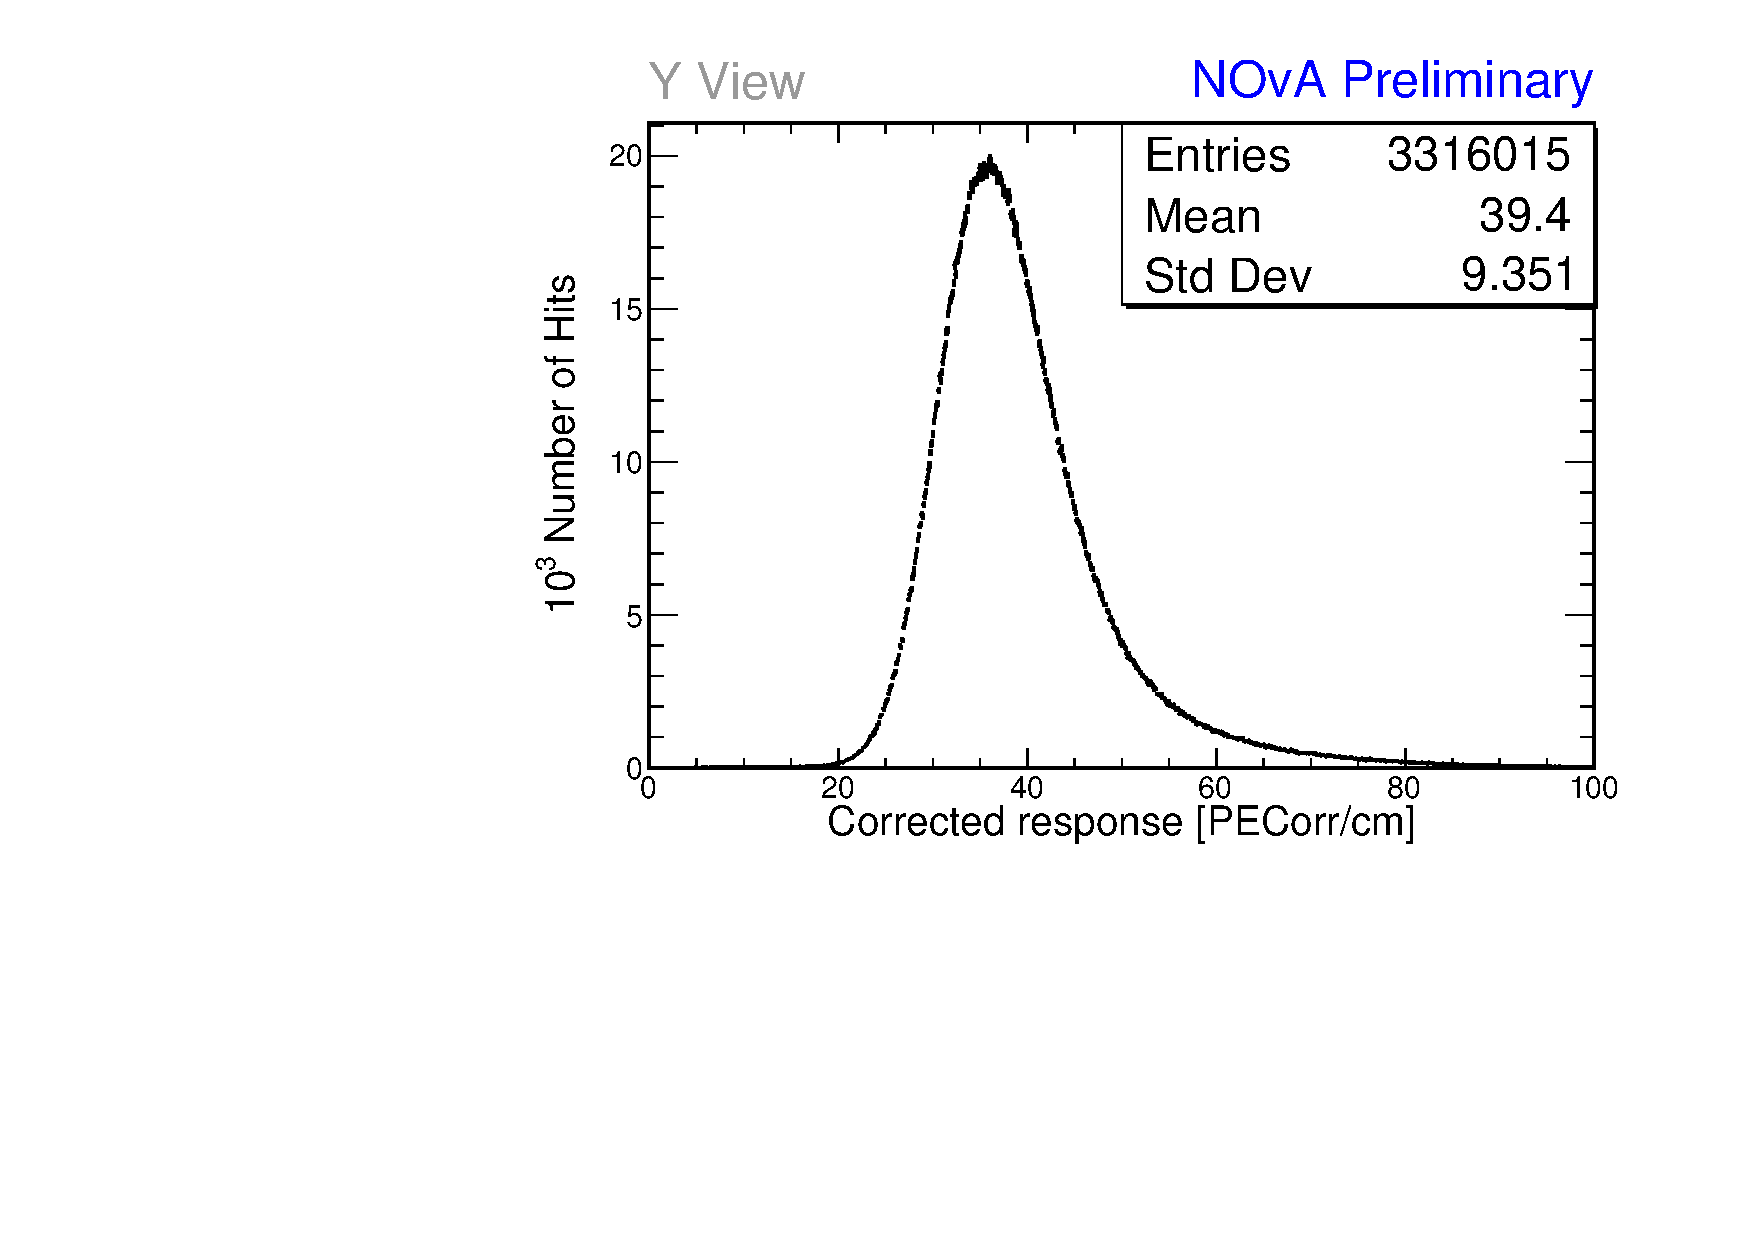
\includegraphics[width=0.49\textwidth]{Plots/NOvAExperiment/ExampleAbsCalib_P4_meu_y.pdf}
    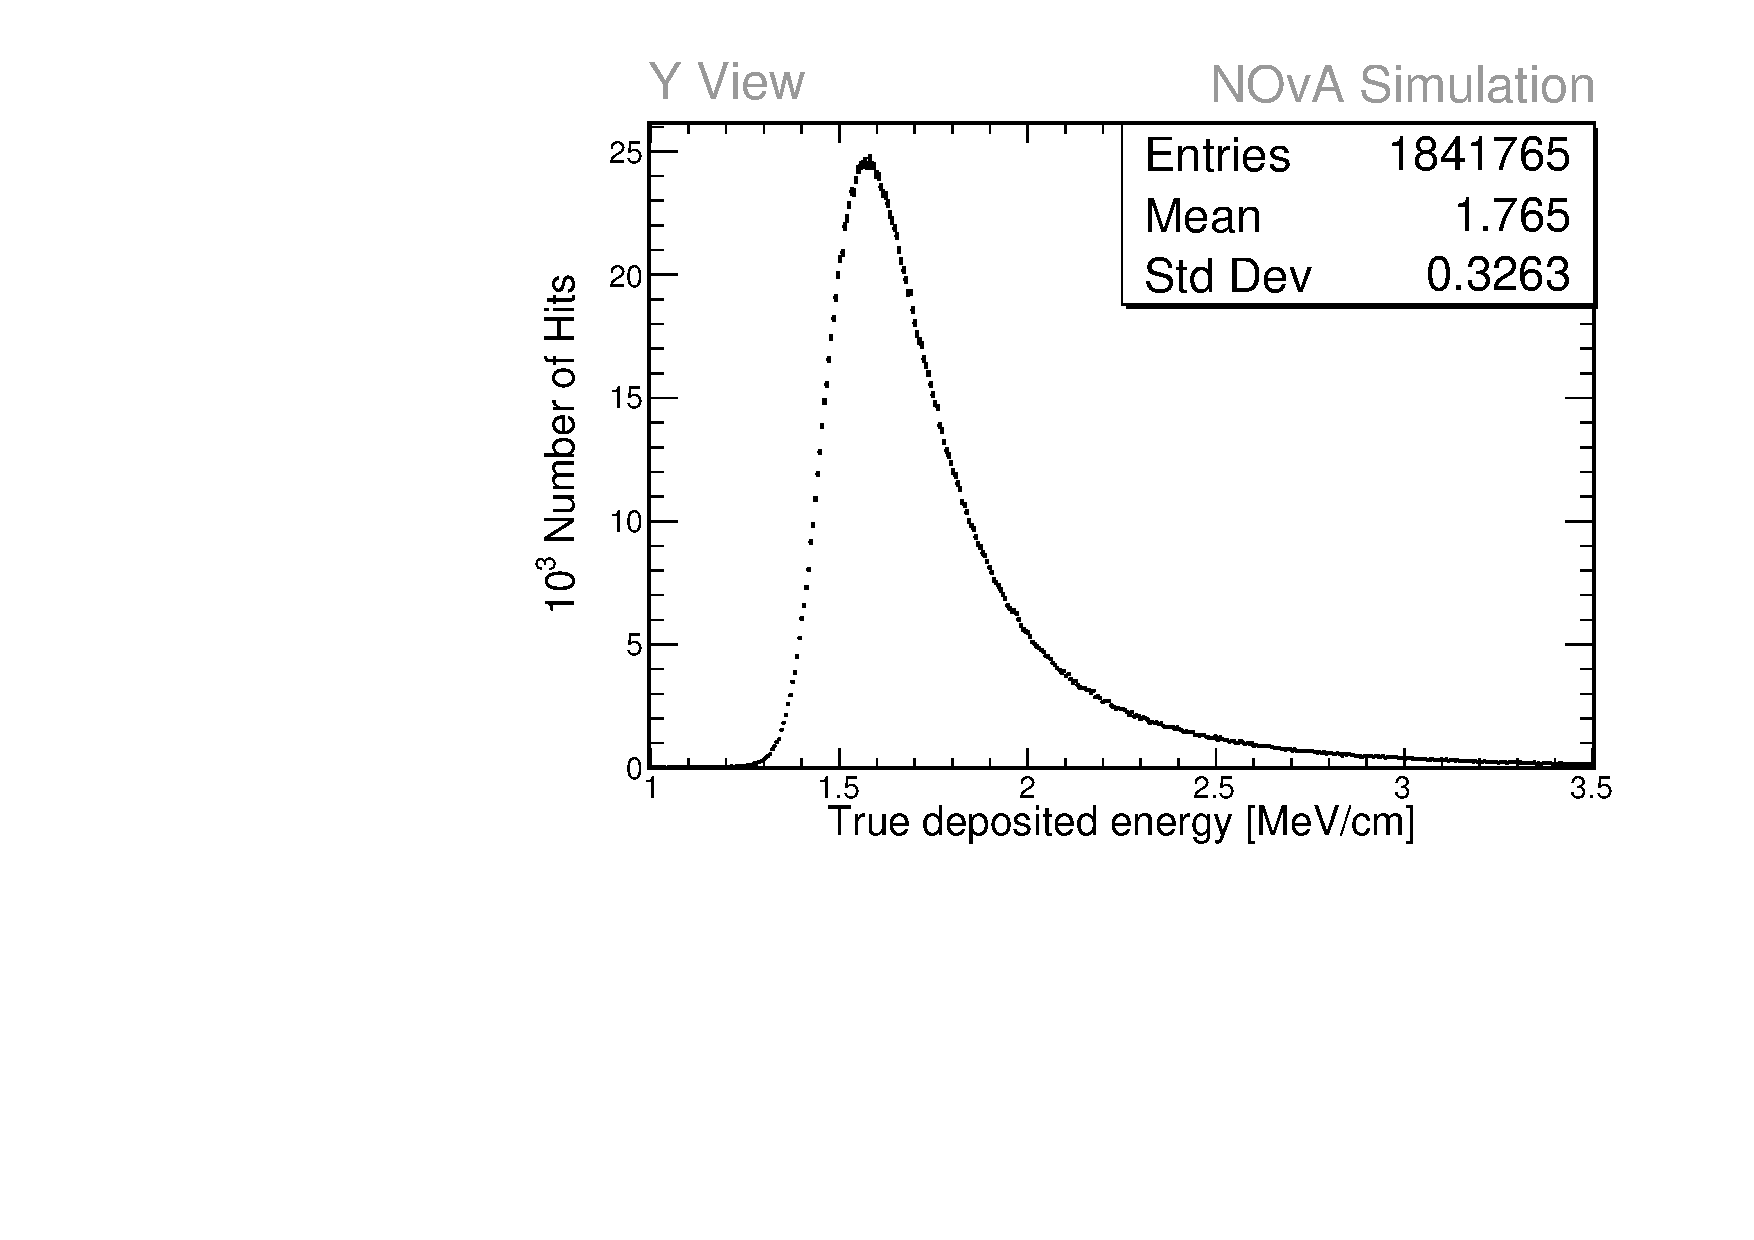
\includegraphics[width=0.49\textwidth]{Plots/NOvAExperiment/ExampleAbsCalib_Sim_mev_y.pdf}
    \caption[Example distributions for the NOvA absolute calibration]{To calculate the absolute energy scale we take the mean reconstructed energy response (left) for selected stopping muons for each view and each data period or simulation, and use it to divide the simulated mean true deposited energy (right).}
    \label{fig:NOvACalibrationAbsoluteEnergyScale}
\end{figure}

%For each calibrated data and simulation sample we take a mean of the corrected deposited energy distribution, separate for each view. We then take a simple average from the two views to get the final $\textsf{MEU}_{reco}$ in units of $\unit{PECorr/cm}$ for each sample \cite{NOvA-doc-13579-FACalorimetricEnergyScale}. Additionally, from simulation we can get the mean of the distribution of the true deposited energy in the scintillator, $\textsf{MEU}_{truth}$ in units of $\unit{MeV/cm}$ for the same sample of stopping muons. 

We save these absolute energy scales, as well as the results of the attenuation fit, in a set of lookup tables, which are used any time a hit is recorded in the NOvA detector and processed through the NOvA data processing algorithms.

%Stopping muons provide a good sample of known energy deposits. If we can collect a “golden” sample, they should provide the scale factor to convert PECorr to GeV. So far, the method used has been imperfect, and the absolute calibration constants are known to be off by approx. 10\%. Since a factor already has to be derived to correct for dead material, this is not significantly impeding current efforts, but work was recently gone into improving this area. [docdb:7410 - this was likely before the track window cut was introduced] (Here it says that it's not such a big a problem since we have to scale for the dead material anyway. But nowadays we have to account for a large systematic uncertainty in the absolute energy scale in our analyses. How is the dead material correction different from the energy scale uncertainty?)

%...the calibration of the calorimetric energy scale of the NOvA detectors uses the energy deposited by stopping muons as a standard candle. To reduce systematic uncertainties, only those energy deposits in a 1-2 m window away from the muon track end point are used. The mean of the detector response distribution is found for data and MC in both near and far detectors. The mean of the distribution of true energy deposits in the track window is used to provide a conversion factor between the detector response and the true energy deposited in the scintillator for minimum ionising muons. The simulated dE/dx is uniform within about 1.8\% for hits around the minimum between 100-200 cm from the track end. The energy that a muon deposits within each cell is estimated using Geant 4 and stored in Fibre Liquid Scintillator (FLS) hits. FLS hits are only those within the active material (liquid scintillator) and energy loss within the passive material (plastic extrusions) is ignored. an estimate of the minimum energy loss rate of stopping muons in the NOvA scintillator is found to be,
%\begin{equation}
%\left.\frac{dE}{dx}\right|_{\textsf{mip}}=\left(1.7915\pm 0.0035\right)\unit{MeV/cm}.
%\end{equation}
%For stopping muons in NOvA it is also important to consider their decay. The muon has a vacuum lifetime of about 2.2 microseconds and favourably decays, with a branching ratio approx. 100\%, into an electron, an electron anti-neutrino and a muon neutrino. The electron produced in this decay is called a Michel electron and is used to select muons that stop within the NOvA detectors. The energy scale calibration is performed using cosmic ray muons. The calibration measures the detector response in data and MC in both near and far detectors and normalises them all by providing a conversion factor, for all four cases, that converts the detector response to energy in GeV. The energy loss rate (dE/dx) of stopping muons is well described by the Bethe-Bloch and is a function of the distance from the stopping point. A track window technique is used to minimise the variations in detector response that depend on the distance to the track end. Using this technique only hits within a region of distances from the track end are used. The position of the track window is chosen such that a mis-reconstruction of the track end point has the minimum effect on the mean detector response. The track window is currently set to be in the range from 100 cm to 200 cm from the track end.[docdb:13579 - FA\_Calorimetric\_energy\_scale]

\section{Energy estimation}
\note{Should I include this section or not?}

%[NOvAResults2021.pdf] Neutrino energy is determined using different methods for the nue and numu CC candidate events. The energies of nue CC candidates are parametrized using a quadratic function determined from a 2D fit to the simulated electromagnetic (EM) and hadronic calorimetric energies (EEM and Ehad respectively). The two components produce different detector responses and are separated using a third CNN classifier that identifies EM-like hit clusters within the event with the remaining clusters being classified as hadronic [80]. For numu CC candidates, Enu is the sum of the muon energy, determined by the track length, and the total calorimetric energy of the hadronic system, Ehad . The muon is identified with a BDT that utilizes track length, multiple Coulomb scattering, and energy deposi tion, while the hadronic system is taken as all hits not associated with the muon track.

%[NOvAResultsCombinedNuAnu2019.pdf] The incident neutrino energy is reconstructed from the measured energies of the final-state lepton and recoil hadronic system. The lepton energy is estimated from track length for muon candidates and from calorimetric energy for electron candidates. The hadronic energy is estimated from the sum of the calibrated hits not associated with the primary lepton. The neutrino energy resolution at the FD is 9.10\% (8.1\%) for numu CC (anumu CC) events and 10.7\% (8.8\%) for nue CC (anue CC) events. We analyze the numu and anumu events in quartiles of hadronic energy fraction as events with less hadronic energy have the best energy resolution and lowest backgrounds [21].

%[NOvAHalfTimeOverview2022.pdf] The energy of charged current neutrino interactions is estimated from the sum of energies of the lepton and the hadronic recoil system. A Kalman-like algorithm is used with a BDT based on energy loss, multiple scattering, and length parameters of a candidate track to identify muons and reconstruct their energy using track length. The energy of electron neutrinos is estimated from a quadratic function, derived from the simulation, of the measured calorimetric energies of the electromagnetic activity and hadronic activity in the event [33, 34].

\section{Systematic Uncertainties at NOvA}\label{sec:NOvASystematics}
\todo{Describe the general systematic uncertainties for NOvA}
\note{These subsections below might end up just being paragraphs, depends how much I want to write about them}

\subsection{Systematic Uncertainties Related to the NOvA Neutrino Beam}

\todo{Describe the Hadron production and focusing systematic uncertainties}

\todo{Principal component analysis}

\note{Maybe briefly also mention the POT scaling normalization uncertainty.}

%From docdb:54582: NOvA analyses use two sets of flux uncertainties: beam transport, which cover differences between the simulation and the working conditions of the NuMI beam, and hadron production, which concern the rates of production of pions and kaons from proton collisions on the carbon target. The beam transport uncertainties include the horn and target position, the horn current, the beam position on the target, the beam spot size, and the effect of the Earth’s magnetic field in the beam pipe (which is not simulated in G4NuMI). The effect of each uncertainty is below 5% at the flux peak for both the ND and FD. PPFX is used to constraint the hadron production models for the NuMI beam using external hadron production data and theory. The systematic effect is assessed by generating 100 universes where the uncertainty on the external data and theoretical assumptions are allowed to float. Flux uncertainties are known to show correlations across most neutrino energy bins, especially in off-axis measurements like NOvA. NOvA looks at 100 PPFX universes, and for each PPFX universe we further sample the beam transport parameters 20 times, creating a total of 2000 universes representing many different possibilities of the flux uncertainty. These universes are used to estimate the bin-to-bin covariances in true energy for each neutrino flavour, detector and beam mode. A Principal Component Analysis (PCA) is applied to the covariance matrices to find sets of uncorrelated shifts - Principal Components (PCs). The covariance matrices for each neutrino flavour and beam mode are calculated in the (ND, FD/ND) basis to represent the approximate extrapolated error at the Far Detector. These are then diagonalized to give the Principal Components, given by the eigenvectors i.e, $PC_i=\sqrt{\lambda_i}v_i$, where $\lambda_i$ represents the $i$-th largest eigenvalue and $v_i$ its corresponding eigenvector. The components are then converted to the (ND, FD) basis. Each PC can be used as a systematic shift in the oscillation fit with a pull of $1\sigma$. By ordering each of the PCs in terms of the magnitude of their eigenvalues, one can also capture most of the information embedded in the covariance matrix with just a few components. Five principal components are used in the oscillation fit. The hadron production uncertainty on the neutrino flux is evaluated using a "multi-universe" technique. This is $\sim 7\%$ at the spectrum peak dominated by interactions where relevant data to be included in the constraining procedure is currently not available (mostly mesons and proton quasi-elastic interactions). Beam transport uncertainties are incorporated by propagating uncertainties in the alignment of beamline elements, including the beam position on the target, the horns current and position, the beam spot size, and the effect of the Earth magnetic field in the decay pipe. The beam optic uncertainty is $\sim 4\%$ at the peak.

\subsubsection{Constraining the Hadron Production Systematic Uncertainty in NOvA}
%Again, should I discuss it here or somewhere else? Maybe not necessary as a full section. Not sure if I should include a discussion on nu-on-e, or low nu studies here, or just PPFX improvements.

\subsection{Systematic uncertainties for NOvA detectors}

\subsubsection{Neutrino interaction systematic uncertainties}

\subsubsection{Energy scale systematic uncertainty}

%WORK IN PROGRESS

%First Analysis systematic uncertainties due to calibration:
%Sources of systematic uncertainty of particular concern are those introduced by residual variations remaining after calibration. Systematic errors are introduced by spatial and temporal variations in detector response. Further, any difference between the two detectors may introduce a relative shift in the energy scale between the detectors. A source of systematic uncertainty can be introduced by mis-reconstructing the end point of the muon track. Such a mis-reconstruction would shift the window within which hits are selected and hence the dE/dx of the muon.  The figure shows that the detector response varies by up to about 60\% over the range from 0 to 500 cm to the track end. This large variation illustrates the importance of careful consideration of the track window position and size. The detector response for both data and MC is minimum at about 130 cm from the track end and is flat to about 1\% in the range from 100 cm to 200 cm from the track end. For a track window starting at 100 cm from the track end, a conservative mis-reconstruction of the track end point by 10cm will shift the start of the track window to between 90cm and 110cm. This shift will alter the MEU value by less than 0.4\% over the range.
%If the calibration procedure was ideal the detector response would not vary with position in either data or MC. The calibration is not ideal and the detector response and recorded simulated energy deposition varies with position of the hit within the detector, such variations will introduce systematic errors. The position of a hit can be defined by the plane, cell within the plane, and distance along the cell (w) of the hit. The variation in detector response and simulated energy deposition vs. plane, cell and w for each view has been studied to quantify the systematic uncertainty introduced by these sources.
%The rise in detector response at the far end of FD y-view cells is an issue with several potential sources. The rise in response may be due to an acceptance effect or a light-level threshold effect among other possibilities. An acceptance effect is where greater energy must be deposited at the far end of the cells so that the light can travel along the fibre, hit the APD and be recorded as a hit. Both an acceptance effect and a light-level effect would introduce a bias towards higher energy hits toward the far end of cells.
%Another source of systematic uncertainty is introduced by the variation in detector response with time. The FD response is stable to about 1\% during the period from October 2014 to March 2015. The ND response needs further study but there was no significant trend over 6 months at 5\%. 
%As mentioned in Section 5, the version (7.1) of the calibration used for first analysis has been adjusted based on studies of muons from beam neutrinos interacting in the detector [8]. A shift of 3.6\% was introduced based on the average response of muons where large sections of the track were used. When only a track window of 100-200cm is used on the beam muons the difference is only 2.7\% [8]. Our best hypothesis for this residual 2.7\% difference is that it is caused by showery events that are present in ND data but not ND MC: it was shown in [9] that doing the calorimetric energy scale calibration using a truncated mean (or a median or a fit to the peak) gave a data/MC ratio that differed by 2.7\% compared to using the untruncated mean as described in this document. A comparison of various cross checks of the calorimetric energy scale was undertaken (in [10] and [11]) and concluded that the nearly 5\% difference between ND data and MC seen in a sample of Michele electrons [12] should be applied as both an absolute and relative shift to the calorimetric energy scale. The difference between the level of calorimetric energy resolution of stopping muons was studied and it was found that data and MC agreed best when an 8\% additional smearing was introduced. Studies for the NuMu analysis indicated that this was a negligible systematic uncertainty [13]. 
%[docdb:13579 - FA\_Calorimetric\_energy\_scale]

\subsubsection{Cell edge calibration systematic uncertainty}

\subsubsection{Detector ageing systematic uncertainty}

\note{Should I include the neutron systematics, muon energy scale systematic, or tau scale systematics? Are these detector systematics? Should find out...}

%Also include Chenerkov and light level tune uncertainties